\documentclass[xcolor=x11names,compress,professionalfonts, aspectratio=169]{beamer}

%% General packages %%%%%%%%%%%%%%%%%%%%%%%%%%%%%%%%%%
\usepackage[utf8]{inputenc}
\usepackage{graphicx}
\usepackage{tikz}
\tikzset{% change default arrow tips
    >=latex
}
\usepackage{ifthen}

\usepackage{nicefrac}

\usepackage{color}
\usepackage[english, french]{babel} %français
\usepackage{amsmath, amssymb, amsfonts, mathtools}
%\usepackage{makeidx}
%\usepackage{graphicx}
%\usepackage{braket} %quantum mechanics
%\usepackage[usenames,dvipsnames]{xcolor} % colors for text
%\usepackage[absolute]{textpos} % to place elements in the page
%\usepackage{tikz} % drawing in LaTeX
%\usetikzlibrary{positioning}
\usepackage{ dsfont } % hollow letters
%% compile child documents using this preamble
%\usepackage{subfiles}
%% compile child files with separate preambles, and include them in the document
%\usepackage{standalone}
%% subfigure
%\usepackage{subcaption}
%% include pdf pages in the document
%\usepackage{pdfpages}
%% hyperlinks
%\usepackage[colorlinks=true, linkcolor=black, citecolor=black]{hyperref}
%% BODY command inside new environments
%\usepackage{environ}
%% lots of nice custom commands for physicists
\usepackage{physics}
\usepackage{forloop}
%% if structures
%\usepackage{xifthen}
%% include figures in text blocs
%\usepackage{wrapfig}
%% algorithms
%\usepackage{algorithmic, algorithm}
%\usepackage{nicefrac}

%%%%%%%%%%%%%%%%%%%%%%%%%%%%%%%%%%%%%%%%%%%%%%%%%%%%%%

\makeatletter
\setbeamertemplate{footline}
{
    \leavevmode%
    \hbox{%
        \begin{beamercolorbox}[wd=.333333\paperwidth,ht=2.25ex,dp=1ex,center]{author in head/foot}%
            \usebeamerfont{author in head/foot}\insertshortauthor
        \end{beamercolorbox}%
                \begin{beamercolorbox}[wd=.333333\paperwidth,ht=2.25ex,dp=1ex,center]{title in head/foot}%
            \usebeamerfont{title in head/foot}\insertshorttitle
        \end{beamercolorbox}%
        \begin{beamercolorbox}[wd=.333333\paperwidth,ht=2.25ex,dp=1ex,right]{date in head/foot}%
            \usebeamerfont{date in head/foot}\insertshortdate{}\hspace*{2em}
            \insertframenumber{} / \inserttotalframenumber\hspace*{2ex} 
        \end{beamercolorbox}}%
        \vskip0pt%
    }
    \makeatother


%% Beamer Layout %%%%%%%%%%%%%%%%%%%%%%%%%%%%%%%%%%
\useoutertheme[subsection=false,shadow]{miniframes}
\useinnertheme{rectangles}

\setbeamertemplate{navigation symbols}{}%remove navigation symbols

\author{Nicolas Macé}

\newcommand{\btVFill}{\vskip0pt plus 1filll}%place an element at the bottom of the page

\usepackage{libertine}
\usepackage[T1]{fontenc}

\setbeamerfont{title like}{shape=\scshape}
\setbeamerfont{frametitle}{shape=\scshape}

\setbeamercolor*{lower separation line head}{bg=DeepSkyBlue4} 
\setbeamercolor*{normal text}{fg=black,bg=white} 
\setbeamercolor*{alerted text}{fg=red} 
\setbeamercolor*{example text}{fg=black} 
\setbeamercolor*{structure}{fg=black} 
 
\setbeamercolor*{palette tertiary}{fg=black,bg=black!10} 
\setbeamercolor*{palette quaternary}{fg=black,bg=black!10} 

\renewcommand{\(}{\begin{columns}}
\renewcommand{\)}{\end{columns}}
\newcommand{\<}[1]{\begin{column}{#1}}
\renewcommand{\>}{\end{column}}

% custom commands and definitions
%------------------ General setup ------------------%
\definecolor{darkblue}{rgb}{0.0,0.0,0.4}
\hypersetup
{
bookmarksopen=true,
pdftitle=Nicolas Macé - Electronic properties of quasicrytals,
pdfauthor=Nicolas Macé, 
pdfsubject=Electronic properties of quasicrytals, %subject of the document
%pdftoolbar=false, % toolbar hidden
pdfmenubar=true, %menubar shown
pdfhighlight=/O, %effect of clicking on a link
colorlinks=true, %couleurs sur les liens hypertextes
pdfpagemode=None, %aucun mode de page
pdfpagelayout=SinglePage, %ouverture en simple page
pdffitwindow=true, %pages ouvertes entierement dans toute la fenetre
linkcolor=darkblue, %couleur des liens hypertextes internes
citecolor=RoyalBlue, %couleur des liens pour les citations
urlcolor=darkblue %couleur des liens pour les url
}

%---------------- Commands ---------------------------%

%%%%%%%%%%%%%% TYPOGRAPHY %%%%%%%%%%%%%%%%%%%%%%%%%%%%%

% id est
\newcommand{\ie}{i.e.}
% eg
\newcommand{\eg}{e.g.}
% small font size
\renewcommand{\ss}[1]{\scriptsize{\text{#1}}}

%%%%%%%%%%%%%% MISC %%%%%%%%%%%%%%%%%%%%%%%%%%%%%%%%%%%%%

% et al
\newcommand{\etal}{\textit{et~al.}\xspace}
% vector notation
\renewcommand{\vec}[1]{\mathbf{#1}}
% the equal sign I use to define something
\newcommand{\define}{\ensuremath{ \overset{\text{def}}{=} }}
% card sine
\DeclareMathOperator{\sinc}{sinc}
% differential element
\renewcommand{\d}[1]{\mathrm{d}#1}
% similar symbol with a limit underneath
\newcommand{\simlim}[1]{\ensuremath{ \underset{#1}{\sim} }}
% alias for omega
\newcommand{\om}{\ensuremath{\omega}}
% local part of the KK wavefunction
\DeclareMathOperator{\loc}{C}
% idos
\newcommand{\idos}{\ensuremath{\text{idos}}}
% hermitian conjugate
\newcommand{\hc}{\ensuremath{\text{H.c}}}
% region on the tiling
\newcommand{\reg}{\ensuremath{\mathcal{R}}}
% generating function of the height stat
\newcommand{\gen}{\ensuremath{Z}}
% volume of a region
\newcommand{\vol}{\ensuremath{\text{Vol}}}
% Ammann-Beenker alias
\newcommand{\AB}{Ammann-Beenker}
% SKK alias
\newcommand{\SKK}{SKK}
% sim symbol with a limit underneath
\newcommand{\simop}[1]{\ensuremath{\underset{#1}{\sim}}}

% differential element
\renewcommand{\d}[1]{\mathrm{d}#1}

\newcommand{\lb}{\ensuremath{\overline{\lambda}}}
\newcommand{\zb}{\ensuremath{\overline{z}}}
% wavefunction dimensions
\newcommand{\wf}{\ensuremath{d^\psi}}
% averaged wavefunction dimensions
\newcommand{\avwf}{\ensuremath{\overline{D^\psi}}}
% local spectral dimensions
\newcommand{\locspec}{\ensuremath{D^\mu}}
% averaged local spectral dimensions
\newcommand{\avspec}{\ensuremath{D^\mu}}
% bold g letter in math mode
\newcommand{\gv}{\ensuremath{\mathbf{g}}}

% log derivative of the wavefunction
\newcommand{\dlogpsi}{\ensuremath{\d \log \psi}}
% average potential
\newcommand{\meanv}{\ensuremath{\langle V \rangle}}
% ceiling function
\DeclarePairedDelimiter{\ceil}{\lceil}{\rceil}
% floor function
\DeclarePairedDelimiter{\floor}{\lfloor}{\rfloor}
% irrational number
\newcommand{\irr}{\ensuremath{\alpha}}
% cut-and-project
\renewcommand{\cp}{C\&P}
% set of the integers
\newcommand{\zahl}{\ensuremath{\mathds{Z}}}
% fractional part function
\DeclarePairedDelimiter{\fpart}{\{}{\}}
% normalized perp position
\newcommand{\nperp}[2]%
	{%
		\ifthenelse{\isempty{#1}}{\ensuremath{\widetilde{x}_\perp}}{\ensuremath{\widetilde{x}_\perp(#1,#2)}}%
	}
% average with angled brackets
\DeclarePairedDelimiter{\avg}{\langle}{\rangle}
% sturmian fucntion (generate a sturmian sequence)
\newcommand{\sturm}[2]{\ensuremath{S_{#1}\left(#2\right)}}
% Heaviside function
\DeclareMathOperator{\heaviside}{Y}
% support of the multifractal spectrum
\newcommand{\supp}{\ensuremath{\Delta_f}}
% variational groundstate
\newcommand{\psivar}{\ensuremath{\psi_\text{var}}}
% preexponential factor for the variational groundstate
\newcommand{\locvar}{\ensuremath{C_\text{var}}}

%%%%%%%%%%%%%%%%% COMMENTS %%%%%%%%%%%%%%%%%%%%%%%%%%%
\newcommand{\nico}[1]{\textcolor{BrickRed}{#1}}
\newcommand{\anu}[1]{\textcolor{NavyBlue}{#1}}
\newcommand{\fred}[1]{\textcolor{OliveGreen}{#1}}

%%%%%%%%%%%%%%%% QUANTUM MECHANICS %%%%%%%%%%%%%%%%%
% energy
\newcommand{\en}{\ensuremath{\varepsilon}}
% Operator
\renewcommand{\op}[1]{\hat{#1}}
% density of states
\DeclareMathOperator{\dos}{\rho}

%%%%%%%%%%%%%%%% ALPHABETS AND WORDS %%%%%%%%%%%
% the A letter
\newcommand{\A}{\ensuremath{\text{A}}}
% the B letter
\newcommand{\B}{\ensuremath{\text{B}}}
% any sequence of letters
\newcommand{\lett}[1]{\ensuremath{\text{#1}}}
% letter couting function: #1 is the word we count in, #2 is the sequence of letters counted
\newcommand{\nb}[2]{\ensuremath{|#1|_{#2}}}
% substitution
\DeclareMathOperator{\sub}{S}
% word (infinite)
\newcommand{\word}{\ensuremath{w}}
% word complexity
\newcommand{\cmplx}[2]%
	{%
		\ifthenelse{\isempty{#1}}{\ensuremath{\Omega}}{\ensuremath{\Omega(#1,#2)}}%
	}

%%%%%%%%%%%%%%% PERIODIC CRYSTALS %%%%%%%%%%%%%%
\newcommand{\kvec}{\ensuremath{\mathbf{k}}}

%%%%%%%%%%%%%%% MULTIFRACTAL ANALYSIS %%%%%%%%%%
\newcommand{\bc}{box-counting}
% mass (or probability measure) defining a fractal set
\DeclareMathOperator{\mass}{\mu}
% q weight
\DeclareMathOperator{\qweight}{\text{M}}
% partition into a set of boxes
\DeclareMathOperator{\boxset}{\mathcal{B}}
% pointwise Hölder exponent
\DeclareMathOperator{\hold}{\alpha}



\begin{document}

\begin{frame}
\title{Thermalization and localization in one-dimensional quantum systems}

\author{Nicolas Macé}

\date{Janurary 30, 2019}

\titlepage

\btVFill
\begin{columns}
  \begin{column}{2cm}
    \centering
    
\includegraphics[width=\columnwidth]{img/title/logo-ups.png}
  \end{column}
  \begin{column}{2cm}
    \centering
    
\includegraphics[width=\columnwidth]{img/title/LPT-LOGO_RVB.jpg}
  \end{column}
\end{columns}
\end{frame}

%\section{Introduction}
%Each section needs a subsection for the small points on top to show up
\subsection{Dummy}

\begin{frame}{Electronic properties of quasicrystals}

Under the supervision of Anuradha Jagannathan

In collaboration with: Michel Duneau, Pavel Kalugin, Rémi Mosseri, Frédéric Piéchon.

\begin{itemize}
	\only<1>{
	\item {\ss{Fractal dimensions of wave functions and local spectral measures on the Fibonacci chain}\\\emph{Macé, Jagannathan, Piéchon, PRB 93 (20), 2016}}
	}

	\only<2>{
	\item \textbf{\ss Fractal dimensions of wave functions and local spectral measures on the Fibonacci chain}\\
	\textbf{\textit{\ss Macé, Jagannathan, Piéchon, PRB 93 (20), 2016}}
	}	
	
	\item {\ss{Quantum simulation of a 2D quasicrystal with cold atoms}\\
	\emph{Macé, Jagannathan, Duneau, Crystals 6 (10), 124}}

	\only<1>{
	\item {\ss{Critical eigenstates and their properties in one-and two-dimensional quasicrystals}\\
	\emph{Macé, Jagannathan, Kalugin, Mosseri, Piéchon, PRB 96 (4), 2017}}
	}
	
	\only<2>{
	\item \textbf{\ss{Critical eigenstates and their properties in one-and two-dimensional quasicrystals}}\\
	\textbf{\textit{\ss Macé, Jagannathan, Kalugin, Mosseri, Piéchon, PRB 96 (4), 2017}}
	}
	
	\item {\ss{Gap structure of 1D cut and project Hamiltonians}\\
	\emph{Macé, Jagannathan, Piéchon, J. Phys.: Conference Series 809 (1), 012023	}}
\end{itemize}

\end{frame}

\begin{frame}{Electronic properties of quasicrystals}
\(
	\<{6cm}
		\centering
		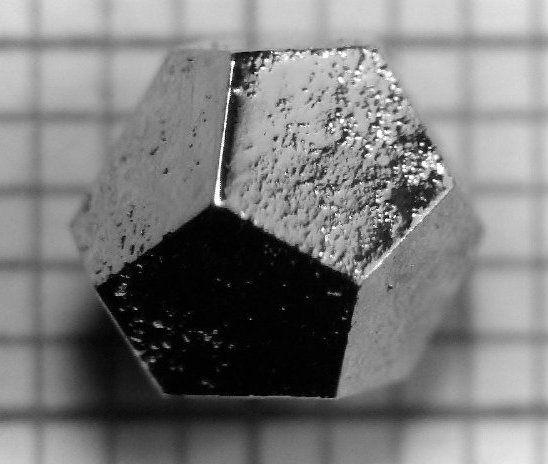
\includegraphics[scale=0.28]{img/1_intro/homgzn.png}
		
		\ss{3D HoMgZn quasicrystalline sample} \ss{(\url{doi:10.1038/nmat1244})}
	\>
	\<{6cm}
		\centering
		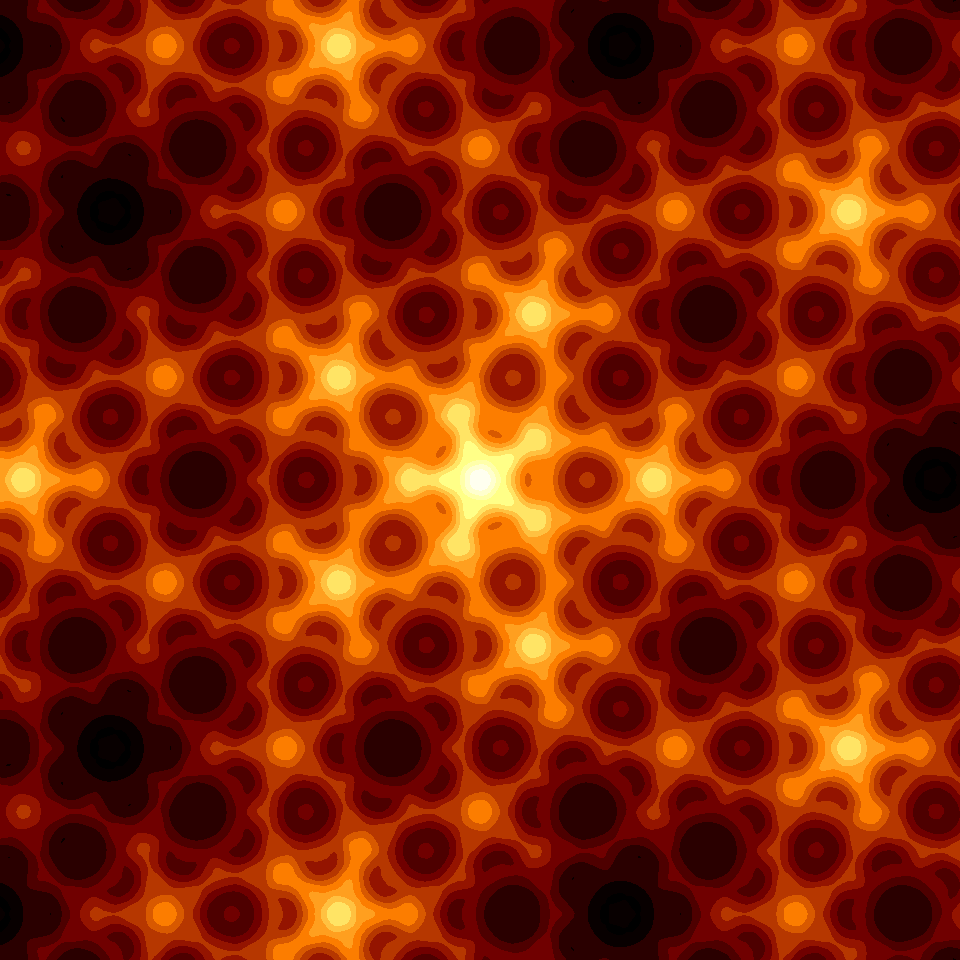
\includegraphics[scale=0.374]{img/1_intro/afmhot}
		
		\ss{Groundstate electron density} \ss{(simple tight-binding model on a 2D tiling)}
	\>
\)
Quasicrystals: not periodic yet ordered structures (discovery: 1982).

Here: single electron properties of tight-binding quasiperiodic models.
\end{frame}

\begin{frame}{A quasiperiodic puzzle [Bédaride \etal{} 12]}

\centering

\includegraphics[width=.4\textwidth]{img/1_intro/tiles_euro.pdf}

Pay the squares, get the rhombuses for free!

\(
\<{6cm}
\centering
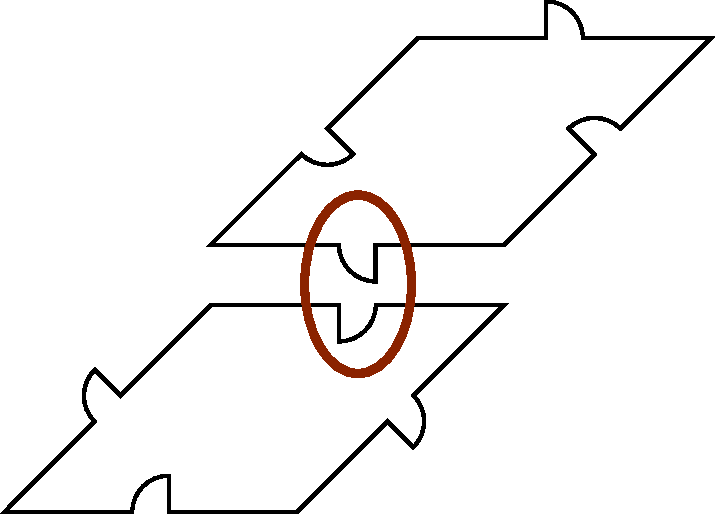
\includegraphics[width=.8\textwidth]{img/1_intro/forbidden.pdf}

Forbidden configuration.
\>

\<{6cm}
\centering

\includegraphics[width=1.\textwidth]{img/1_intro/ammann.pdf}

Patch of the Ammann-Beenker tiling.
\>
\)
\end{frame}

\begin{frame}{Periodic, quasiperiodic and random}
\only<1>{
A random tiling:

\centering

\includegraphics[width=.4\textwidth]{img/1_intro/random00.pdf}

}

\only<2>{
Two copies of the tiling:

\centering

\includegraphics[width=.75\textwidth]{img/1_intro/random01.pdf}

}

\only<3>{
\centering
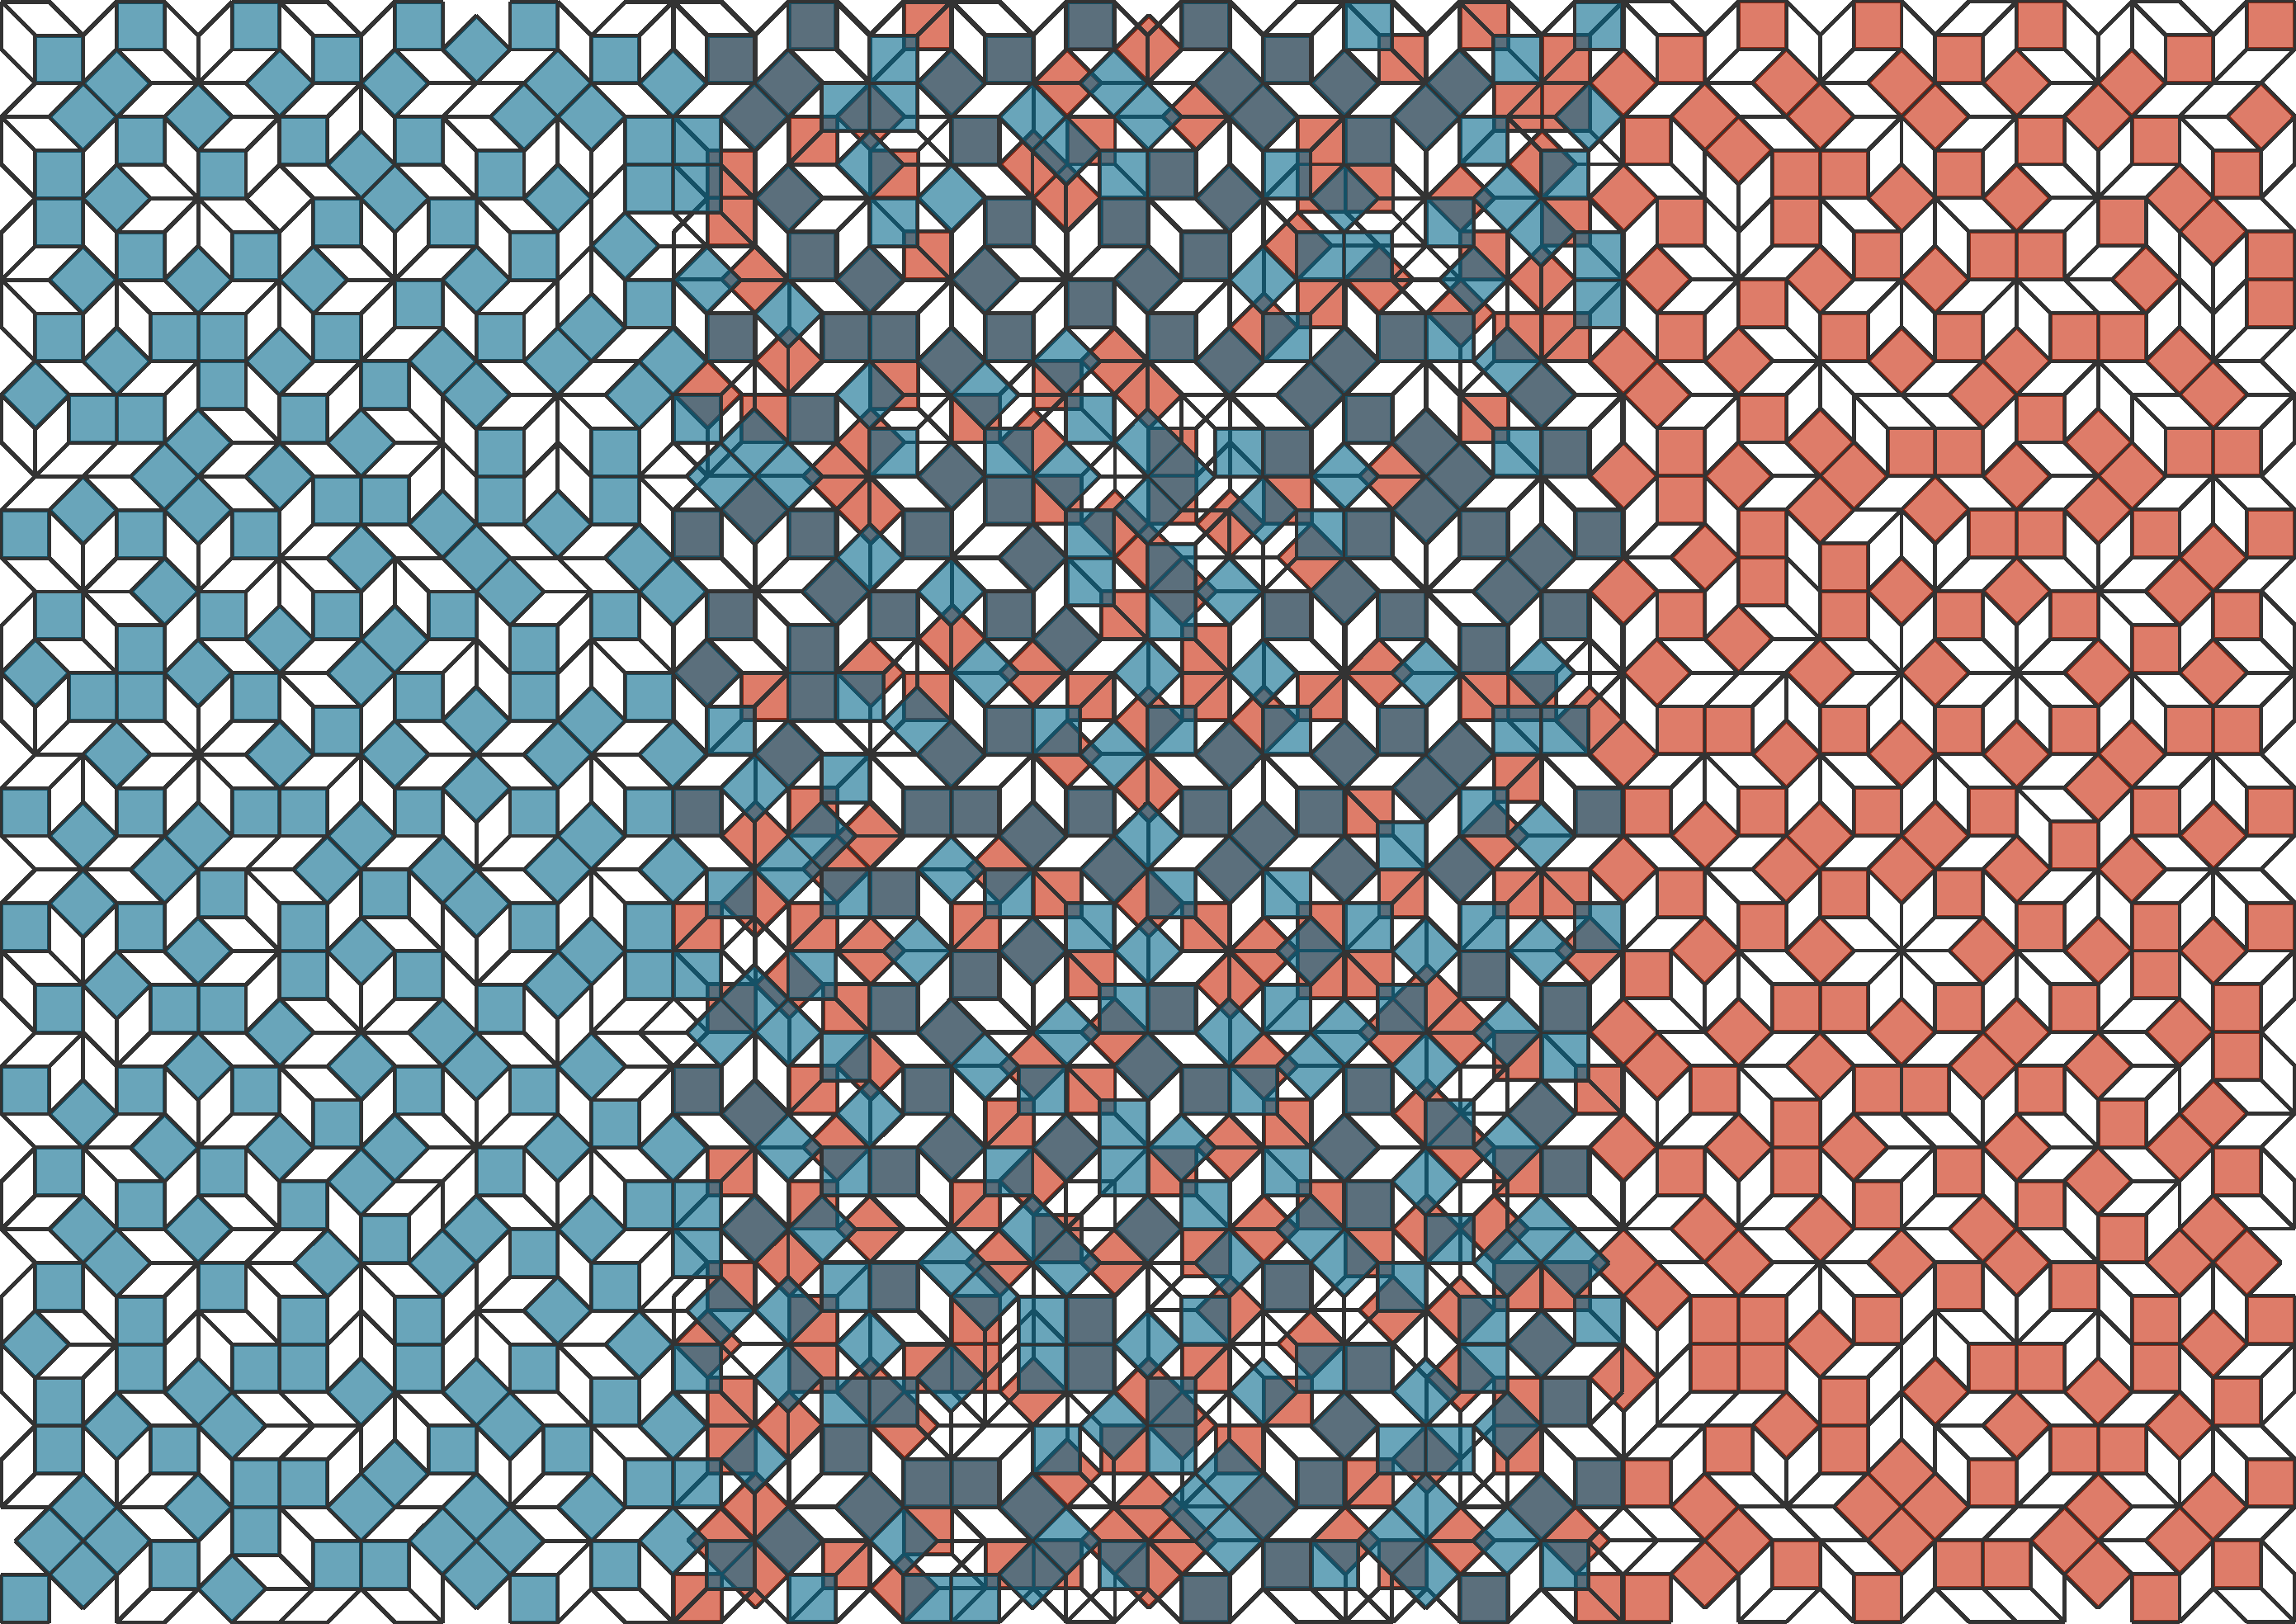
\includegraphics[width=.6\textwidth]{img/1_intro/random.pdf}

$\to$ no overlap $\to$ no order}

\centering
\only<4>{
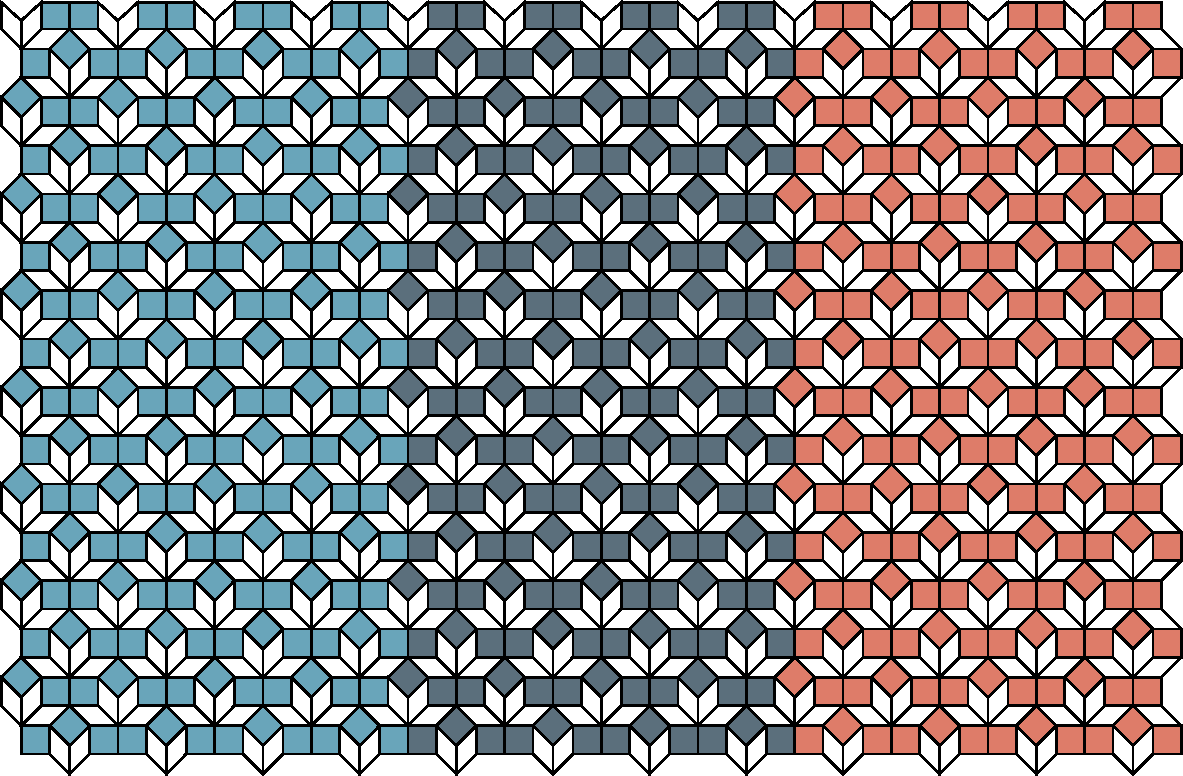
\includegraphics[width=.6\textwidth]{img/1_intro/periodic.pdf}

Perfect long range order: periodic}

\only<5>{

\includegraphics[width=.6\textwidth]{img/1_intro/quasiperiodic.pdf}

Long range order: quasiperiodic 

\flushleft{(see Chap.\ 2 of [Grimm, Baake 13])}
}

\end{frame}

%\begin{frame}{From tiles to atoms}
%Place atoms at the vertices of the tiling:
%
%{\centering
%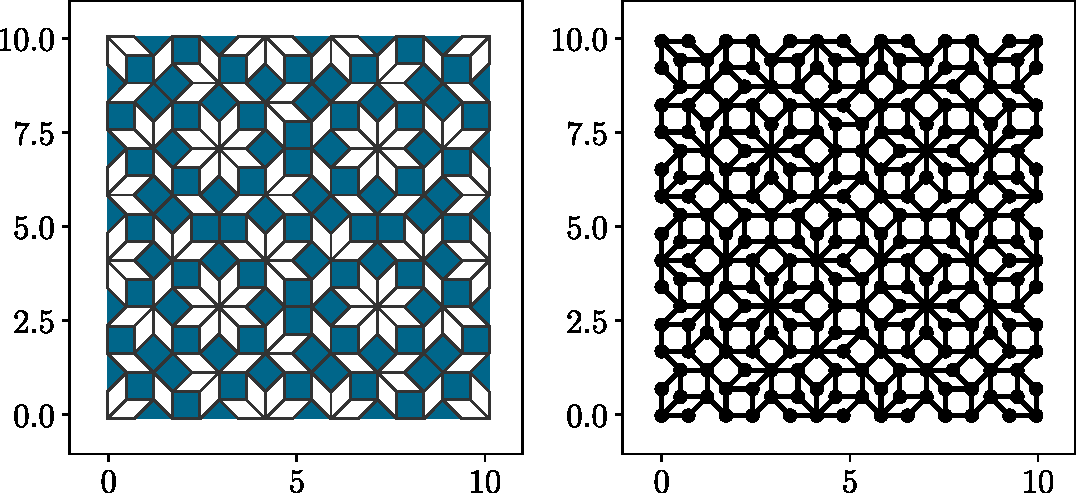
\includegraphics[width=.6\textwidth]{img/1_intro/AB_tiling_and_plot.pdf}
%
%}
%
%$\rightarrow$ can atoms arrange in such a quasiperiodic fashion?
%\end{frame}

\begin{frame}{Quasicrystals}
Quasicrystal $\to$ quasiperiodically arranged atoms:
\begin{itemize}
	\item \textbf{aperiodicity}
	\item \textbf{long range order} (diffraction pattern exhibits sharp peaks).
\end{itemize}
\(
	\<{6cm}
		\centering
		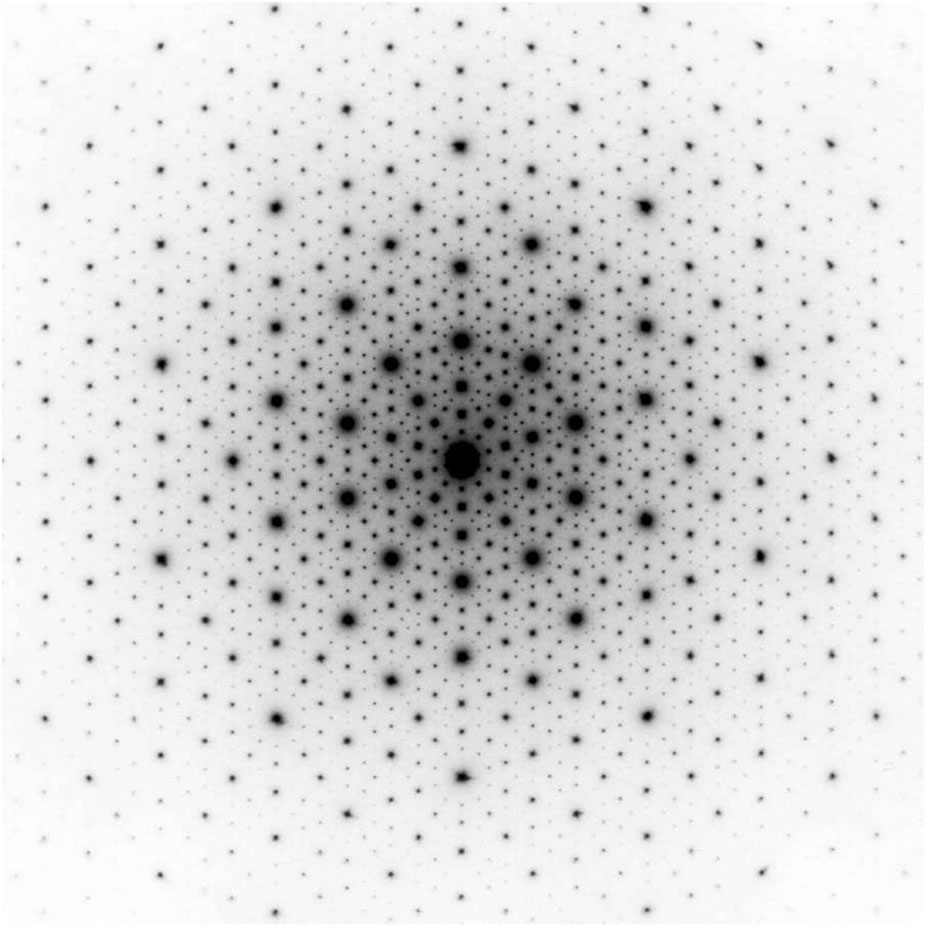
\includegraphics[scale=0.1]{img/1_intro/diffraction_tenfold.png}
		
		\ss{Diffraction pattern of a AlPdMn alloy} \ss{(Conradin Beeli group)}
	\>
	\<{6cm}
		\centering
		
\includegraphics[scale=0.06]{img/1_intro/penrose.png}
		
		\ss{A patch of the quasiperiodic Penrose tiling,} \ss{used to model many quasicrystals.}
	\>
\)
\end{frame}

\begin{frame}{Artificial quasiperiodic structures}
\centering
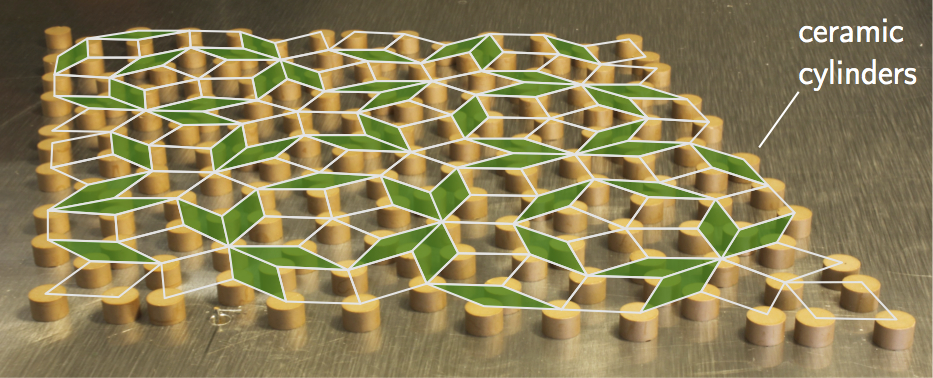
\includegraphics[width=.5\textwidth]{img/1_intro/dielectric_resonators.png}

{\ss{A network of dielectric resonators [Vignolo \etal{} 14]}}

\begin{itemize}
	\item Plasmons in semiconductor stacks [Merlin \etal{} 85]
	\item Microwaves in perforated metallic films [Matsui \etal{} 07]
	\item Microwaves in dielectric resonator networks [Vignolo \etal{} 14]
	\item Light solitons [Freedman \etal{} 07]
	\item Cold atoms in laser potentials [Guidoni \etal{} 97]
	\item Polaritons in wire cavities [Tanese \etal{} 14]
\end{itemize}
\end{frame}


\begin{frame}{Fractals}
Fractal: object invariant under rescaling
\(
\<{7cm}
\centering
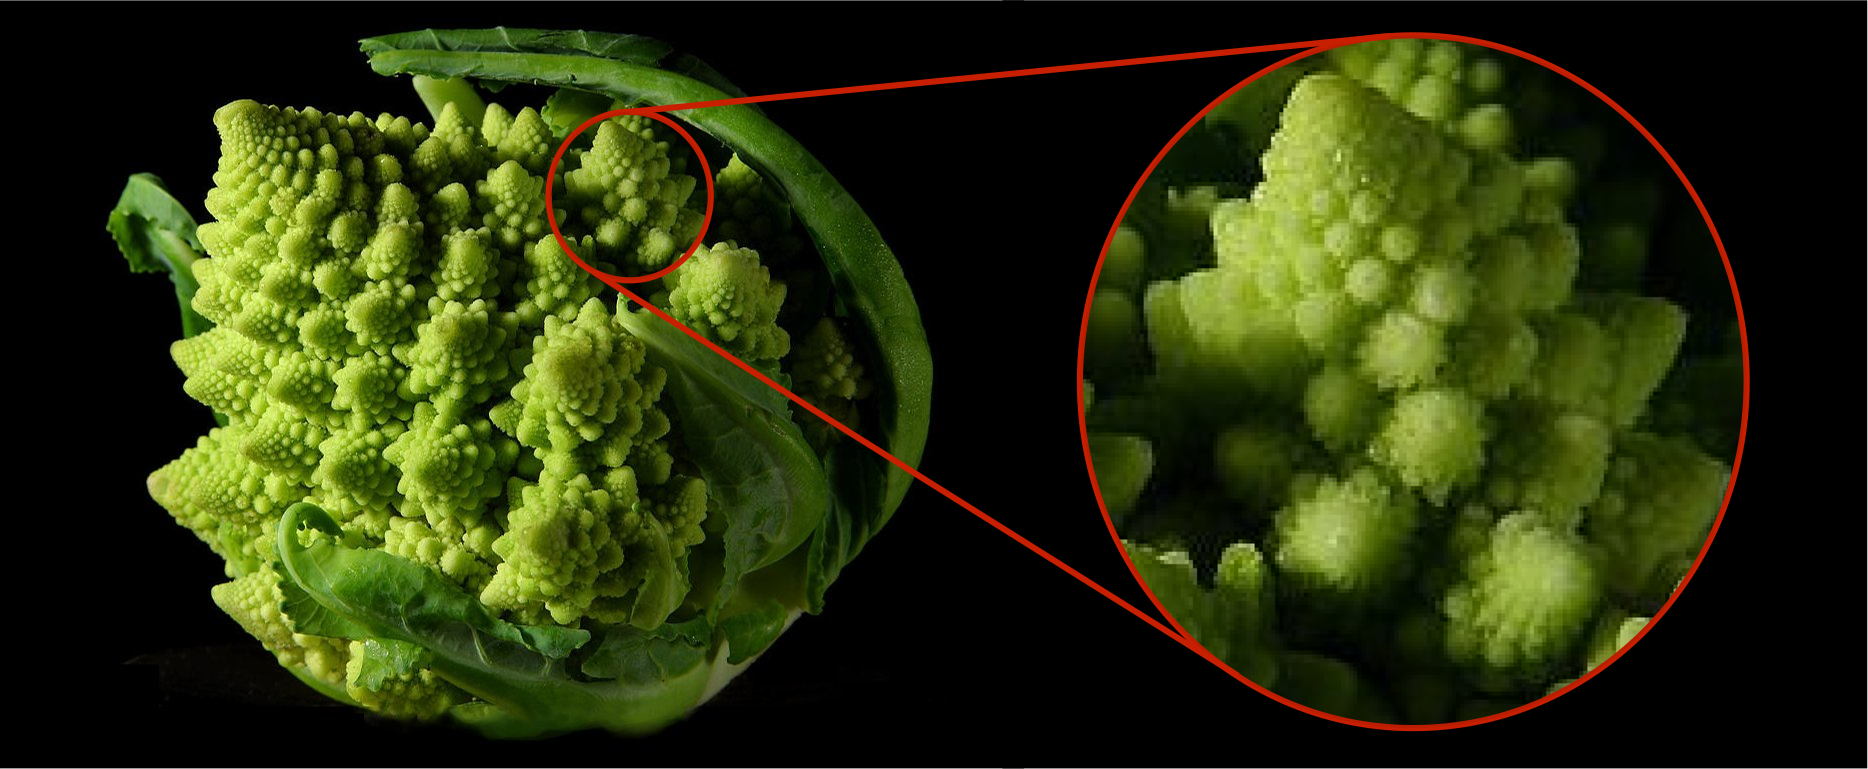
\includegraphics[width=1.\textwidth]{img/1_intro/Fractal_Broccoli.png}

{\ss Romanesco broccoli (\copyleft{} Wikimedia commons)}
\>
\<{7cm}
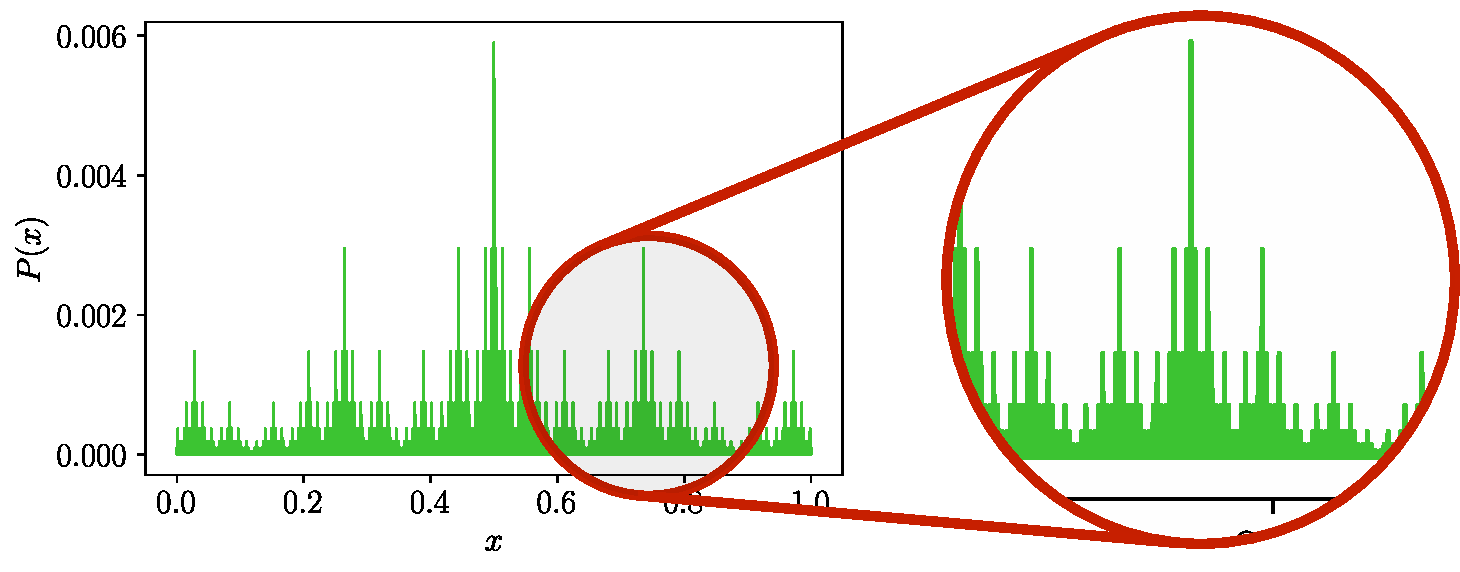
\includegraphics[width=1.\textwidth]{img/1_intro/heights.pdf}

{\ss Electronic density along a quasiperiodic chain}
\>
\)

Quasicrystals \emph{not} fractal\dots

\dots but electrons on quasicrystals $\to$ fractal behavior

\begin{beamerboxesrounded}%
        [shadow=true]%
        {Goal:}
\textbf{Link the fractal behavior of the electrons to quasiperiodicity}
\end{beamerboxesrounded}
\end{frame}

\begin{frame}{Fractal dimensions}
\begin{itemize}
	\item $M(L) \propto L^d$ for a non-fractal $d$-dimensional object\dots What happens for a fractal one?
	
	{\centering
	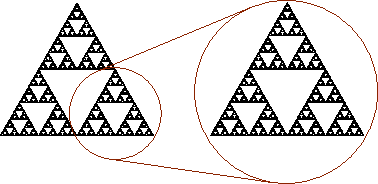
\includegraphics[width=.4\textwidth]{img/2_part1/sierpinski}
	
	{\ss A Sierpiński triangle}
	
	}
	
	\[
		M(L) \sim L^{d_0} \text{, with } d_0 = \log 3/\log 2
	\]
	
	\item $d_0$ is the Hausdorff fractal dimension
	\item $1 < d_0 \simeq 1.58 < 2$, signature of a fractal object
	\item Probe fractality of the $q^\text{th}$ moment of a distribution $\to$ generalized fractal dimensions $d_q$.
\end{itemize}
\end{frame}
%\section{Fibonacci chain}
\subsection{Dummy}
\begin{frame}{The Fibonacci chain}
\(
\<{7cm}{\textbf{Fibonacci numbers}}

A simple rule for generating numbers:
\begin{align*}
	F_0 &= 1 \\
	F_1 &= 1 \\
	F_2 &= F_1 + F_0 = 2 \\
	F_3 &= F_2 + F_1 = 3 \\
	F_4 &= F_3 + F_2 = 5 \\
	F_5 &= F_4 + F_3 = 8 \\
	&\vdots
\end{align*}
\[
	F_{l+2} = F_{l+1} + F_l
\]

\>

\<{7cm}{\textbf{Fibonacci words}}

Letters instead of numbers, same rule:
\begin{align*}
	C_0 &= \B \\
	C_1 &= \A \\
	C_2 &= C_1C_0 = \lett{AB} \\
	C_3 &= C_2 C_1 = \lett{ABA} \\
	C_4 &= C_3 C_2 = \lett{ABAAB} \\
	C_5 &= C_4 C_3 = \lett{ABAABABA} \\
	&\vdots
\end{align*}
\[
	C_{l+2} = C_{l+1}C_l
\]
\>
\)
\end{frame}

% counter has to be defined outside of the frame, otherwise a new counter is created at each iteration of only
\newcounter{slideno}
\begin{frame}{Fibonacci word from above}
(Infinite) Fibonacci word: \ca\cb\ca\ca\cb\ca\cb\ca\ca\cb\ca\ca\cb\dots

\ca{} $\leftrightarrow$ horizontal step, \cb{} $\leftrightarrow$ vertical step

\centering
\forloop{slideno}{1}{\value{slideno} < 14}{%
\only<\theslideno>{\includegraphics[width=.7\textwidth]{img/2_part1/CP_fibo_\theslideno}}%
}
\end{frame}

\begin{frame}{Quasiperiodicity of the Fibonacci word}
\(
\<{9cm}
\centering
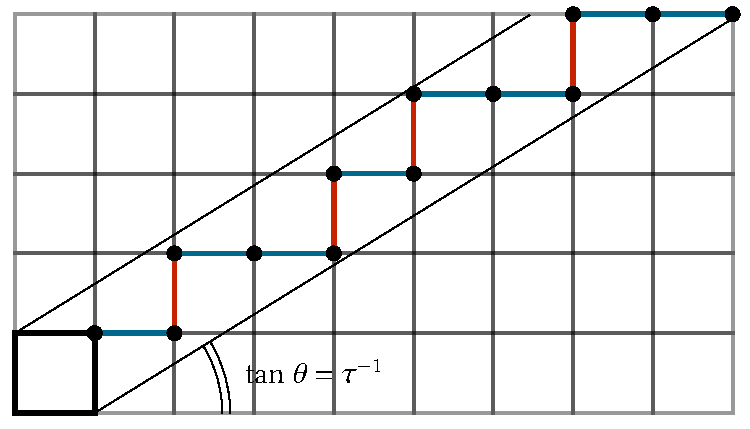
\includegraphics[width=1.\textwidth]{img/2_part1/CP_fibo_cut}
\>
\<{6cm}
\begin{itemize}
	\item average slope = inverse of the golden ratio ($\tau \simeq 1.6$)
	\item bounded fluctuations
\end{itemize}
$\to$ similar environments everywhere

$\to$ quasiperiodicity [Duneau, Katz 85]
\>
\)
\end{frame}

\begin{frame}{Cut-and-project}
\(
\<{9cm}
\centering
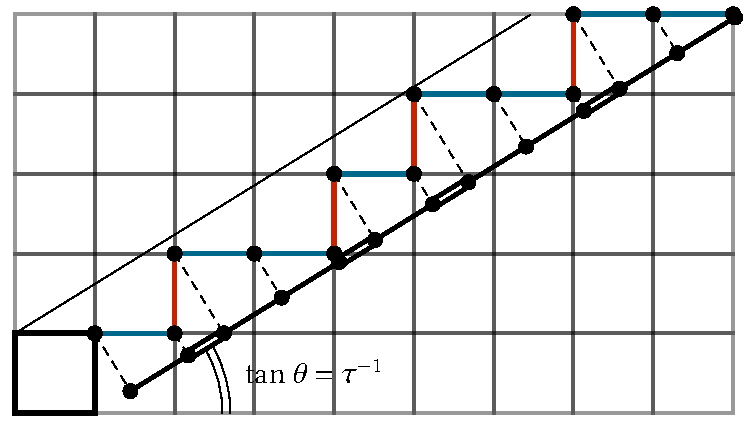
\includegraphics[width=1.\textwidth]{img/2_part1/full_cp}
\>
\<{6cm}
The cut-and-project algorithm:
\begin{enumerate}
	\item choose a hypercubic lattice (here $\zahl^2$)
	\item choose a ``physical plane'' $E_\parallel$ (here a slope)
	\item select points by translating the unit hypercube along $E_\parallel$
	\item project them onto $E_\parallel$.
\end{enumerate}
\>
\)

\textbf{\cp{} $\to$ quasiperiodic (or periodic) tiling!}
\end{frame}

\begin{frame}{From letters to atoms}
\begin{itemize}
	\item The Fibonacci word:
	\ca\cb\ca\ca\cb\ca\cb\ca\dots
	
	\item The Fibonacci (tight-binding) chain of atoms:
	
	{\centering
	%\documentclass[draft.tex]{subfiles}
%\documentclass{standalone}
%\usepackage{tikz}
%\begin{document}


    	\begin{tikzpicture}[scale=.6]
    		\newcommand{\orig}{-1.5}
    		\newcommand{\trans}{1.5}
    		\newcommand{\vertspac}{-2.}    		
    		\newcommand{\rad}{2pt} % radii of the circles
    		
    		% set the style of the strong bonds
    		\tikzset{
    			strong/.style={
    				double,
    				double distance=\rad,
    				line width=0.5pt
    				}
    		}
    	
    		% initial chain
    	
    		% bonds 
			\draw[-] (\orig+\trans,0) -- (\orig+2*\trans,0) node [midway, above] {$t_\ca$};
			\draw[strong] (\orig+2*\trans,0) -- (\orig+3*\trans,0) node [midway, above] {$t_\cb$};	
			\draw[-] (\orig+3*\trans,0) -- (\orig+4*\trans,0) node [midway, above] {$t_\ca$};
			\draw[-] (\orig+4*\trans,0) -- (\orig+5*\trans,0) node [midway, above] {$t_\ca$};
			\draw[strong] (\orig+5*\trans,0) -- (\orig+6*\trans,0) node [midway, above] {$t_\cb$};
			\draw[-] (\orig+6*\trans,0) -- (\orig+7*\trans,0) node [midway, above] {$t_\ca$};
			\draw[strong] (\orig+7*\trans,0) -- (\orig+8*\trans,0) node [midway, above] {$t_\cb$};
			\draw[-] (\orig+8*\trans,0) -- (\orig+9*\trans,0) node [midway, above] {$t_\ca$};
    	
    	
    		% sites
		    \filldraw (\orig+1*\trans,0) circle (\rad);% node [below] {6};
		    \filldraw (\orig+2*\trans,0) circle (\rad);% node [below] {3};
		    \filldraw (\orig+3*\trans,0) circle (\rad);% node [below] {8};
		    \filldraw (\orig+4*\trans,0) circle (\rad);% node [below] {5};
		    \filldraw (\orig+5*\trans,0) circle (\rad);% node [below] {2};
		    \filldraw (\orig+6*\trans,0) circle (\rad);% node [below] {7};
		    \filldraw (\orig+7*\trans,0) circle (\rad);% node [below] {4};
		    \filldraw (\orig+8*\trans,0) circle (\rad);% node [below] {1};
		    \filldraw (\orig+9*\trans,0) circle (\rad) node [right] {\dots};
		      
		\end{tikzpicture}

%\end{document}%
	}

\end{itemize}
Hamiltonian:
\[
	\op{H} = - \sum_m t_m \ket{m-1} \bra{m} + \hc
\]
Schrödinger equation for the eigenstate of energy $E$:
\[
	E \psi(m) = -t_{m}\psi(m-1) -t_{m+1}\psi(m+1)
\]
\end{frame}

\begin{frame}{The broccoli $E=0$ state}
\(
\<{6cm}
\centering
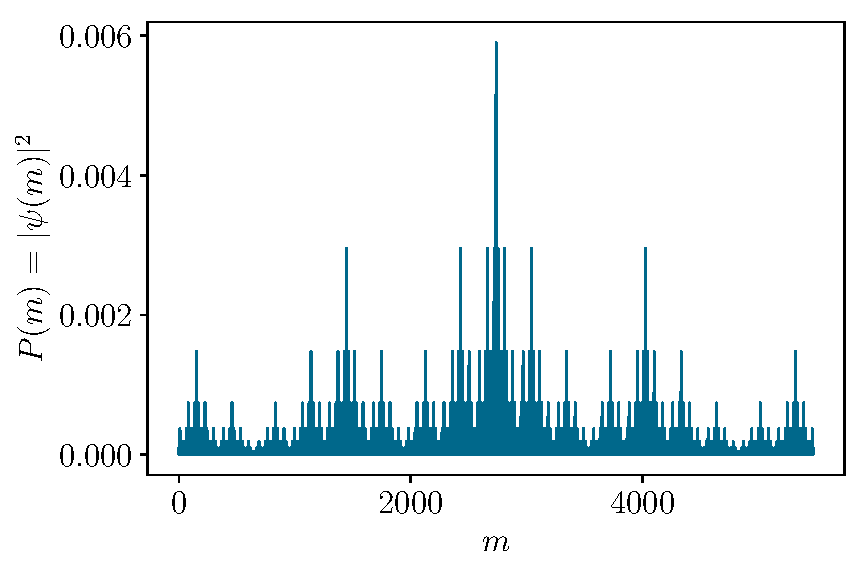
\includegraphics[width=1.\textwidth]{img/2_part1/state_fibo}

{\ss ``Romanesco broccoli'' fractal state at energy $E=0$}
\>
\<{8cm}
\begin{itemize}
	\item State at 0 energy verifies
	\[ t_m \psi(m-1) + t_{m+1}\psi(m+1) = 0 \]
	\item Fibonacci chain decouples into two chains:
	
	{\centering	
	\documentclass[../talk.tex]{subfiles}
\begin{document}


    	\begin{tikzpicture}[scale=.7]
    		\newcommand{\orig}{-1.5}
    		\newcommand{\trans}{1.5}
    		\newcommand{\vertspac}{-2.}
    		\newcommand{\vertsize}{0} % vertical span of the rectangles
    		\newcommand{\del}{.2}
    		\newcommand{\rad}{2pt} % radii of the circles

    		
    		% set the style of the strong bonds
    		\tikzset{
    			strong/.style={
    				double,
    				double distance=\rad,
    				line width=0.5pt
    				}
    		}
    	
    		% initial chain
    	
    		% bonds 
        	\draw[-] (\orig, 0)  node [left] {...}  -- (\orig+\trans, 0) node [midway, below] {};
			\draw[strong] (\orig+\trans,0) -- (\orig+2*\trans,0) node [midway, below] {};
			\draw[-] (\orig+2*\trans,0) -- (\orig+3*\trans,0) node [midway, below] {};	
			\draw[strong] (\orig+3*\trans,0) -- (\orig+4*\trans,0) node [midway, below] {};
			\draw[-] (\orig+4*\trans,0) -- (\orig+5*\trans,0) node [midway, below] {};
			\draw[-] (\orig+5*\trans,0) -- (\orig+6*\trans,0) node [midway, below] {};
			\draw[strong] (\orig+6*\trans,0) -- (\orig+7*\trans,0) node [midway, below] {};
			\draw[-] (\orig+7*\trans,0) -- (\orig+8*\trans,0) node [right] {...} node [midway, below] {};
    	
    		% sites
			\filldraw (\orig+0*\trans,0) circle (\rad) node [below] {$h=0$} node [above] {$\psi=1$};
			\filldraw (\orig+1*\trans,0) circle (\rad) node [below] {};
			\filldraw (\orig+2*\trans,0) circle (\rad) node [below] {$h=1$} node [above] {$\psi=\rho$};
			\filldraw (\orig+3*\trans,0) circle (\rad) node [below] {};
			\filldraw (\orig+4*\trans,0) circle (\rad) node [below] {$h=2$} node [above] {$\psi = \rho^2$};
			\filldraw (\orig+5*\trans,0) circle (\rad) node [below] {};
			\filldraw (\orig+6*\trans,0) circle (\rad) node [below] {$h=2$} node [above] {$\psi = \rho^2$};
			\filldraw (\orig+7*\trans,0) circle (\rad) node [below] {};
			\filldraw (\orig+8*\trans,0) circle (\rad) node [below] {$h=1$} node [above] {$\psi = \rho$};
			
			% arrow
			\path[->] (\orig+0*\trans,0) edge[bend right = 80] node [below] {+1} (\orig+2*\trans,0);
			\path[->] (\orig+2*\trans,0) edge[bend right = 80] node [below] {+1} (\orig+4*\trans,0);
			\path[->] (\orig+4*\trans,0) edge[bend right = 80] node [below] {+0} (\orig+6*\trans,0);
			\path[->] (\orig+6*\trans,0) edge[bend right = 80] node [below] {-1} (\orig+8*\trans,0);

		\end{tikzpicture}

\end{document}
	}

	\item Work on groups of two letters:
	\begin{itemize}
		\item \ca\cb{} $\leftrightarrow$ R
		\item \cb\ca{} $\leftrightarrow$ L
		\item \ca\ca{} $\leftrightarrow$ U
	\end{itemize}
	
\end{itemize}
\>
\)
\end{frame}

\begin{frame}{Structure of the broccoli}
\(
\<{8cm}
\begin{itemize}
	\item Effective chain
	\[
		\underbrace{\ca\cb}_{R}\underbrace{\ca\ca}_{U}\underbrace{\cb\ca}_{L}\underbrace{\cb\ca}_{L}\underbrace{\ca\cb}_{R}\underbrace{\ca\ca}_{U}\dots
	\]
	\item \textbf{Arrow function}: $A(R) = +1$, $A(L) = -1$, $A(U) = 0$.
	\item \textbf{Height function}: $h(m) = \sum_{n \leq m} A_n$
	\item Let $\rho = t_\cb/t_\ca$.
	\[
		\boxed{
		\psi(m) = (-1)^m \rho^{h(m)}
		}
	\]
\end{itemize}
\>
\<{8cm}
\centering
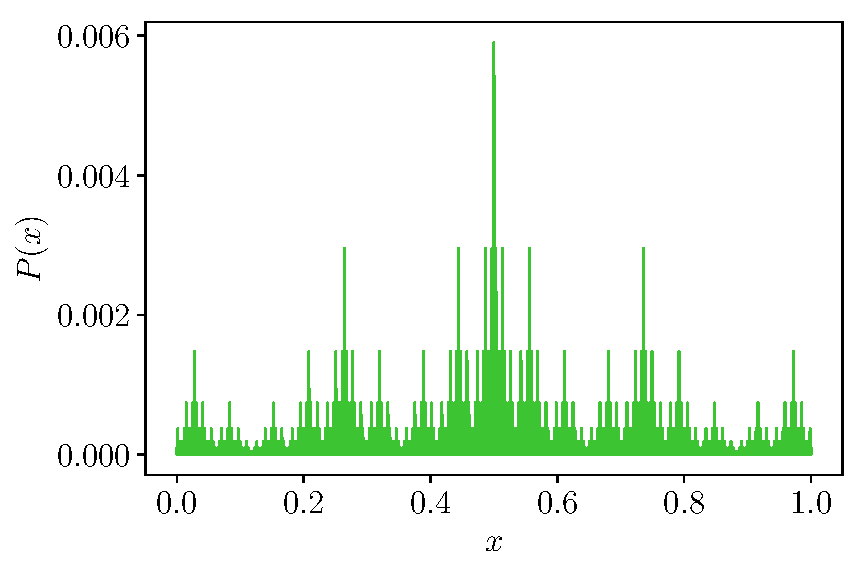
\includegraphics[width=.7\textwidth]{img/2_part1/heights_fibo}

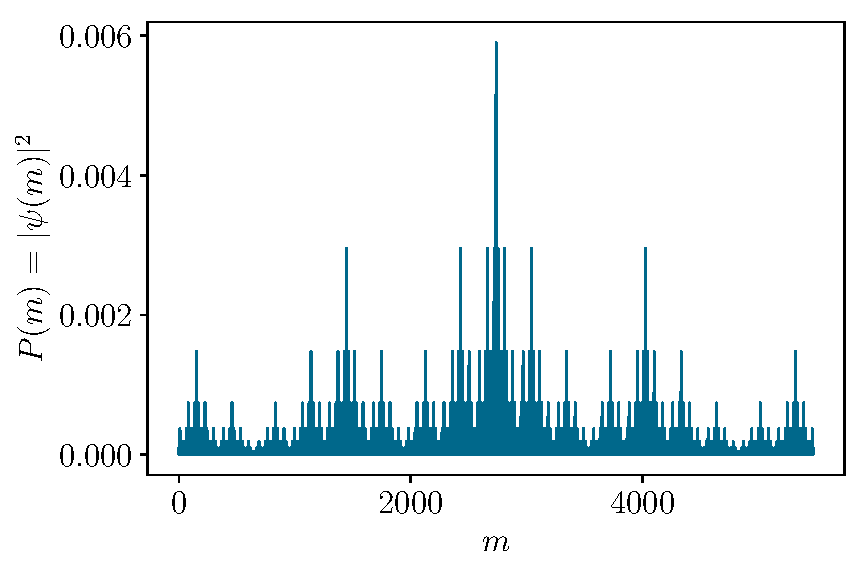
\includegraphics[width=.65\textwidth]{img/2_part1/state_fibo}
\>
\)
\end{frame}

\begin{frame}{Geometry and eigenstate properties}
\(
\<{8cm}
\begin{itemize}
	\item Arbitrary chain \ca\ca\ca\cb\cb\ca\cb\cb\dots{} (not necessarily Fibonacci)
	\item $E=0$ state: $\psi(m) = (-1)^m \rho^{h(m)}$
	\item Geometry $\leftrightarrow$ $h(m)$ function
\end{itemize}

\begin{itemize}
	\item Periodic chain: \ca\ca\ca\ca\ca\dots
%	\documentclass[../talk.tex]{subfiles}
\begin{document}

		\begin{tikzpicture}[scale=.7]
    		\newcommand{\orig}{-1.5}
    		\newcommand{\trans}{1.5}
    		\newcommand{\vertspac}{-2.}
    	
    		% initial chain
    	
    		% bonds 
        	\draw[-] (\orig+\trans,0) -- (\orig+2*\trans,0) node [midway, above] {};
			\draw[-] (\orig+2*\trans,0) -- (\orig+3*\trans,0) node [midway, above] {};	
			\draw[-] (\orig+3*\trans,0) -- (\orig+4*\trans,0) node [midway, above] {};
			\draw[-] (\orig+4*\trans,0) -- (\orig+5*\trans,0) node [midway, above] {};
			\draw[-] (\orig+5*\trans,0) -- (\orig+6*\trans,0) node [midway, above] {};
			\draw[-] (\orig+6*\trans,0) -- (\orig+7*\trans,0) node [midway, above] {};
			\draw[-] (\orig+7*\trans,0) -- (\orig+8*\trans,0) node [midway, above] {};
			\draw[-] (\orig+8*\trans,0) -- (\orig+9*\trans,0) node [midway, above] {};
			
			% wavefunction
			%\draw (\orig+4*\trans,0) -- (\orig+6*\trans,0) node [midway, above] {$\psi(r) = e^{ik r}$};
    	
    		% sites
		    \filldraw (\orig+1*\trans,0) circle (0.05) node [left] {...};
		    \filldraw (\orig+2*\trans,0) circle (0.05) node [below] {};
		    \filldraw (\orig+3*\trans,0) circle (0.05) node [below] {};
		    \filldraw (\orig+4*\trans,0) circle (0.05) node [below] {};
		    \filldraw (\orig+5*\trans,0) circle (0.05) node [below] {};
		    \filldraw (\orig+6*\trans,0) circle (0.05) node [below] {};
		    \filldraw (\orig+7*\trans,0) circle (0.05) node [below] {};
		    \filldraw (\orig+8*\trans,0) circle (0.05) node [right] {};
		    \filldraw (\orig+9*\trans,0) circle (0.05) node [right] {...};
		      
		\end{tikzpicture}
		
\end{document}
	\begin{itemize}
		\item Arrows $= 0 \implies |\psi(m)| = $ cst  
		\item \textbf{extended state}
	\end{itemize}
	\item Disordered chain: \ca\ca\ca\cb\cb\ca\cb\cb\dots
%	%\documentclass[../talk.tex]{subfiles}
%\begin{document}

\begin{tikzpicture}[scale=.7]
    		\newcommand{\orig}{-1.5}
    		\newcommand{\trans}{1.5}
    		\newcommand{\vertspac}{-2.}
    		 \newcommand{\rad}{2pt} % radii of the circles
    		 
    		% set the style of the strong bonds
    		\tikzset{
    			strong/.style={
    				double,
    				double distance=\rad,
    				line width=0.5pt
    				}
    		}
    	
    		% initial chain
    	
    		% bonds 
        	\draw[strong] (\orig+\trans,0) -- (\orig+2*\trans,0) node [midway, above] {};
			\draw[-] (\orig+2*\trans,0) -- (\orig+3*\trans,0) node [midway, above] {};	
			\draw[strong] (\orig+3*\trans,0) -- (\orig+4*\trans,0) node [midway, above] {};
			\draw[strong] (\orig+4*\trans,0) -- (\orig+5*\trans,0) node [midway, above] {};
			\draw[strong] (\orig+5*\trans,0) -- (\orig+6*\trans,0) node [midway, above] {};
			\draw[-] (\orig+6*\trans,0) -- (\orig+7*\trans,0) node [midway, above] {};
			\draw[-] (\orig+7*\trans,0) -- (\orig+8*\trans,0) node [midway, above] {};
			\draw[-] (\orig+8*\trans,0) -- (\orig+9*\trans,0) node [midway, above] {};
			
			% wavefunction
			%\draw (\orig+4*\trans,0) -- (\orig+6*\trans,0) node [midway, above] {$\psi(r) = e^{- r/\xi}$};
    	
    		% sites
		    \filldraw (\orig+1*\trans,0) circle (0.05) node [left] {...};
		    \filldraw (\orig+2*\trans,0) circle (0.05) node [below] {};
		    \filldraw (\orig+3*\trans,0) circle (0.05) node [below] {};
		    \filldraw (\orig+4*\trans,0) circle (0.05) node [below] {};
		    \filldraw (\orig+5*\trans,0) circle (0.05) node [below] {};
		    \filldraw (\orig+6*\trans,0) circle (0.05) node [below] {};
		    \filldraw (\orig+7*\trans,0) circle (0.05) node [below] {};
		    \filldraw (\orig+8*\trans,0) circle (0.05) node [right] {};
		    \filldraw (\orig+9*\trans,0) circle (0.05) node [right] {...};
		      
		\end{tikzpicture}
%\end{document}
	\begin{itemize}
		\item Random arrows $\implies |\psi(m)| \sim e^{- m^\alpha/\xi}$
		\item \textbf{localized state}
	\end{itemize}
\end{itemize}
\>
\<{8cm}
\begin{itemize}
	\item Quasiperiodic chain
	\begin{itemize}
		\item Discrete scale invariance:
	
		{\centering
		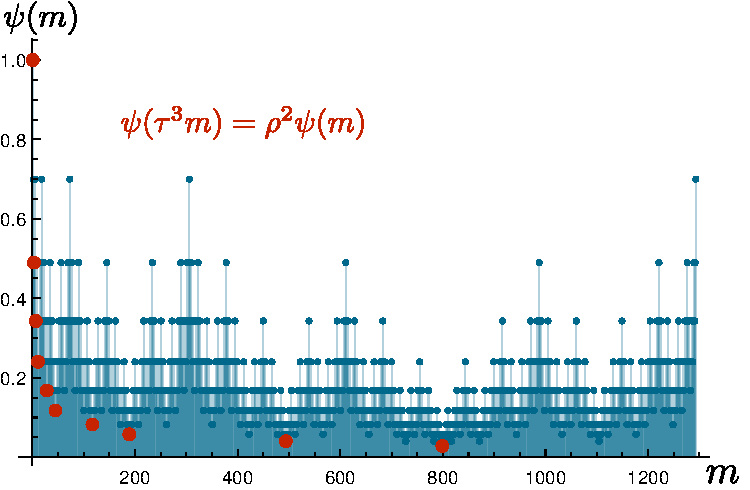
\includegraphics[width=.7\textwidth]{img/2_part1/power_law_decay}}
	
		\item Local power-law behavior $\textcolor{comp}{|\psi(m)| \sim m^{-\alpha}}$
		\item \textbf{critical state} [Kohmoto \etal{} 87]
	\end{itemize}
\end{itemize}
\>
\)
\end{frame}

\begin{frame}{Underlying scale invariance}
Fibonacci chain \emph{itself} scale invariant?

\(
\<{7cm}
\begin{itemize}
	\item Fibonacci words by concatenation:\\
	$C_2 = \lett{AB}$ \\
	$C_3 = \lett{ABA}$ \\
	$C_4 = C_3 C_2 = \lett{ABAAB}$
	
	\item Fibonacci words by \textbf{substitution}:
	\[
		\sub: 
		\begin{cases}
			\A \to \lett{AB}\\
			\B \to \A.
		\end{cases}
	\]
	$C_3 = \lett{ABA}$ \\
	$C_4 = S(C_3) = 
	\only<1>{\sub(\A)\sub(\B)\sub(\A)}
	\only<2>{\lett{AB}\sub(\B)\sub(\A)}
	\only<3>{\lett{AB}\A\sub(\A)}
	\only<4>{\lett{AB}\A\lett{AB}}
	$
\end{itemize}
\>
\<{7cm}
\begin{itemize}
	\item Infinite chain = fixed point of the substitution: \\
	$S(\lett{ABAAB}\dots) = \lett{ABAAB}\dots$
	\item Geometric substitution:
	
	{\centering
	    	\begin{tikzpicture}[scale=.6]
    		\newcommand{\orig}{-1.5}
    		\newcommand{\s}{1.5} % length of short bonds
    		\renewcommand{\L}{2.4} % length of long bonds
    		\newcommand{\golden}{1.61}
    		\newcommand{\rs}{\golden*\s} % length of renormalized short bonds
    		\newcommand{\rL}{\golden*\L} % length of renormalized long bonds
    		\newcommand{\vertspac}{2.}    		
    		\newcommand{\rad}{2pt} % radii of the circles
    		\newcommand{\del}{0.2}
    		
    		% set the style of the strong bonds
    		\tikzset{
    			strong/.style={
    				double,
    				double distance=\rad,
    				line width=0.5pt
    				}
    		}
    	
    		%%%%%%%%%% initial chain
    		% bonds 
			\draw[-] (\orig,\vertspac) -- (\orig+\rL,\vertspac) node [midway, below] {$\A$};
			\draw[strong] (\orig+\rL,\vertspac) -- (\orig+\rs+\rL,\vertspac) node [midway, below] {$\B$};	
    		% sites
		    \filldraw (\orig,\vertspac) circle (\rad);% node [below] {6};
		    \filldraw (\orig+\rL,\vertspac) circle (\rad);% node [below] {3};
		    \filldraw (\orig+\rs+\rL,\vertspac) circle (\rad) node [right] {\dots};% node [below] {8};
		        
    		%%%%%%%%% renormalized chain
    		% bonds 
			\draw[-] (\orig,0) -- (\orig+\L,0) node [midway, below] {$\A$};
			\draw[strong] (\orig+\L,0) -- (\orig+\s+\L,0) node [midway, below] {$\B$};	
			\draw[-] (\orig+\s+\L,0) -- (\orig+\s+2*\L,0) node [midway, below] {$\A$};
%			\draw[-] (\orig+2*\s+2*\L,0) -- (\orig+2*\s+3*\L,0) node [midway, below] {$\A$};
%			\draw[strong] (\orig+2*\s+3*\L,0) -- (\orig+3*\s+3*\L,0) node [midway, below] {$\B$};
%			\draw[-] (\orig+3*\s+3*\L,0) -- (\orig+3*\s+4*\L,0) node [midway, below] {$\A$};
%			\draw[strong] (\orig+3*\s+4*\L,0) -- (\orig+4*\s+4*\L,0) node [midway, below] {$\B$};
    	
    		% sites
		    \filldraw (\orig,0) circle (\rad);% node [below] {6};
		    \filldraw (\orig+\L,0) circle (\rad);% node [below] {3};
		    \filldraw (\orig+\s+\L,0) circle (\rad);% node [below] {8};
		    \filldraw (\orig+\s+2*\L,0) circle (\rad) node [right] {\dots};% node [below] {5};
%		    \filldraw (\orig+2*\s+3*\L,0) circle (\rad);% node [below] {2};
%		    \filldraw (\orig+3*\s+3*\L,0) circle (\rad);% node [below] {7};
%		    \filldraw (\orig+3*\s+4*\L,0) circle (\rad);% node [below] {4};
%		    \filldraw (\orig+4*\s+4*\L,0) circle (\rad);% node [below] {1};

		    % arrows below rectangles
		    \draw [<-] (\orig,\del) -- (\orig,\vertspac-\del) node [midway, left] {$\times \frac{1}{\tau}$};
		    \draw [<-] (\orig+\rL,\del) -- (\orig+\rL,\vertspac-\del);
		    \draw [<-] (\orig+\rs+\rL,\del) -- (\orig+\rs+\rL,\vertspac-\del);
		      
		\end{tikzpicture}
	}
	
	\item \textbf{Infinite chain scale invariant}, scaling factor $1/\tau$.
	
\end{itemize}
\>
\)
\end{frame}

\begin{frame}{Height distribution \& multifractality}
\(
\<{7cm}
Partition function of the heights:
\[
	Z_L(\beta) = \sum_{m \in \reg(L)} e^{-\beta h(m)}
\]
Scaling law behavior:
\[
	Z_L(\beta) \simop{L \to \infty} L^{\omega(\beta)}
\]
with
\[
	\om(\beta) = \frac{\sinh^{-1}(1+\cosh(\beta))}{2+\sqrt{5}}
\]
$\to$ access to the distribution of heights
\>
\<{7cm}
Height diffuses slowly through the chain:
\[
	h_\text{typ}(L) \sim \sqrt{\log L}
\]

Fractal dimensions of the $E=0$ state:
\[
	d_q = \frac{q \om(2\kappa) - \om(2\kappa q)}{q-1},~\text{with }\kappa = |\log \rho|
\]
$0 < d_q < 1$ $\to$ \textbf{fractal state}

\flushright{[Macé \etal{} 17]}
\>
\)

\end{frame}

\begin{frame}{Beyond quasiperiodicity}
\(
\<{7cm}
\(
\<{4cm}
B3 chain:
\[
	\sub: 
	\begin{cases}
		\A \to \lett{ABBB}\\
		\B \to \A.
	\end{cases}
\]

Unbounded fluctuations

$\to$ \textbf{not quasiperiodic}

[Frank, Robinson 08]
\>
\<{3cm}
\centering
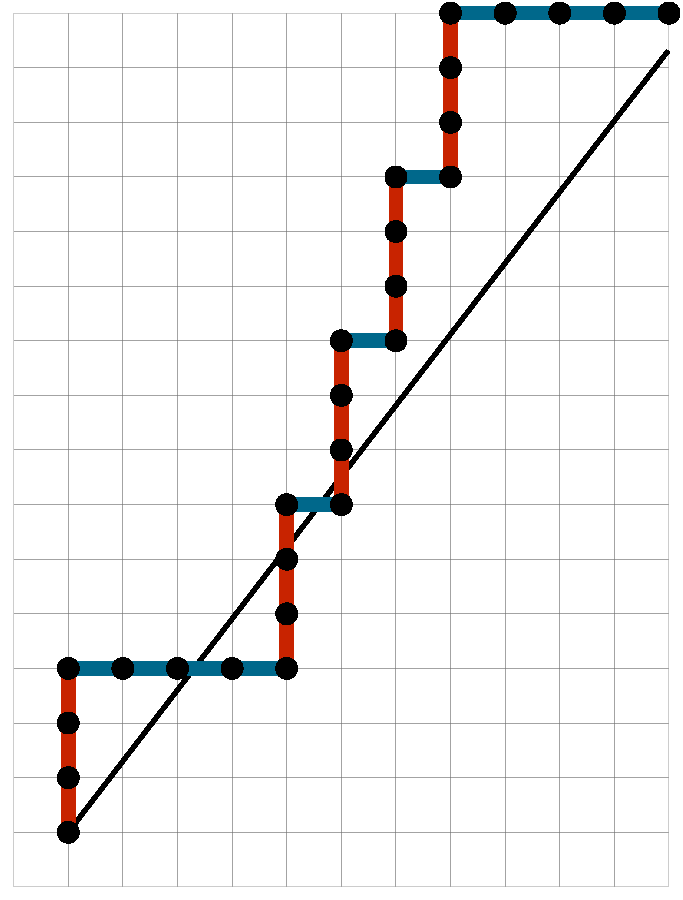
\includegraphics[width=1.\textwidth]{img/2_part1/CP_b3_cut}
\>
\)
\>
\<{7cm}

{\centering
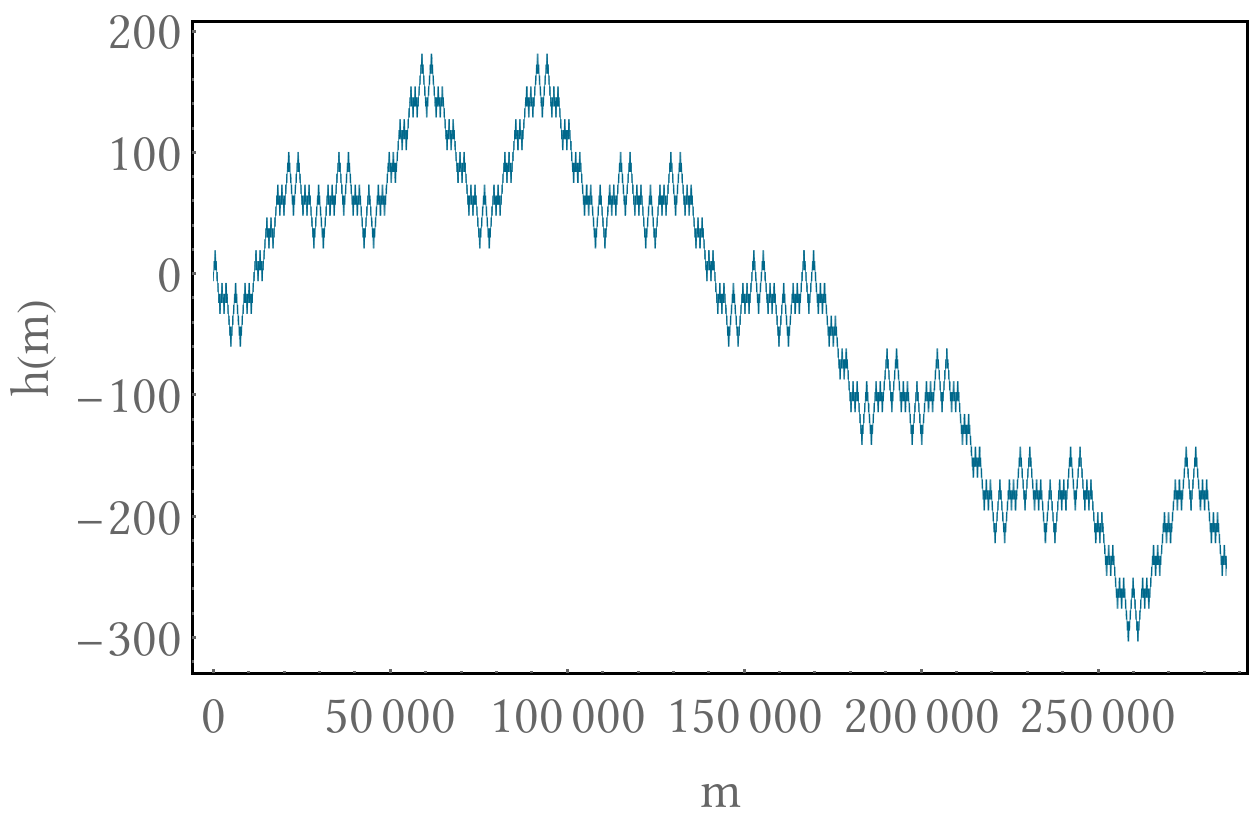
\includegraphics[width=.7\textwidth]{img/2_part1/7_height_b3}

}

Height: power-law growth [Dumont 89]
\[
h(m) = C(m)m^\alpha
\]
%$C$: log-periodic function.

$\to$ \textbf{non-fractal, localized state}
\[
	|\psi(m)| \simop{m \to \infty} e^{-m^\alpha/\xi}
\]
\>
\)
\end{frame}

\begin{frame}{Conclusions}
$E=0$ state of \textcolor{BostonBlue}{two}-\textcolor{comp}{letters} tight-binding chains:
\begin{itemize}
	\item Height field $h(m)$ $\to$ $\psi(m) = (-1)^m \rho^{h(m)}$
\end{itemize}
Effect of the (dis)order:
\begin{itemize}
	\item \textbf{Periodic} $\to$ no height growth $\to$ \textbf{extended} state
	\item \textbf{Quasiperiodic} $\to$ slow height growth ($h(L) \sim \sqrt{\log L})$ $\to$ critical, \textbf{fractal} state
	\item \textbf{Random}/deterministic non-qp $\to$ fast height growth ($h(L) \sim L^\alpha$) $\to$ \textbf{localized} state
\end{itemize}
\end{frame}

\section{Renormalization group on the Fibonacci chain}
\subsection{Dummy}

\begin{frame}{Renormalization group on the Fibonacci chain}
Focused on the $E=0$ state\dots

{\centering
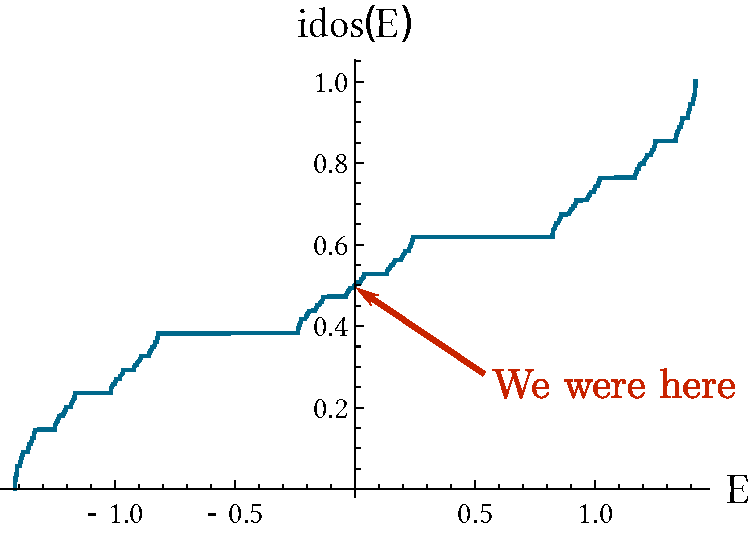
\includegraphics[width=.5\textwidth]{img/3_part2/idos_fibo}

{\ss Integrated density of states (IDoS) of the Fibonacci chain}

}

\dots what about the rest of the spectrum?
\end{frame}

\begin{frame}{Atoms and molecules}
Fibonacci chain in the limit $\rho = t_\A/t_\B = 0$:

{\centering
    	\begin{tikzpicture}[scale=.6]
    		\newcommand{\orig}{-1.5}
    		\newcommand{\trans}{1.5}
    		\newcommand{\vertspac}{-2.}    		
    		\newcommand{\rad}{2pt} % radii of the circles
    		\newcommand{\hh}{1.} % half height of the rectangle
    		\newcommand{\del}{.2} % distance between nodes and border of the rectangle

    		% set the style of the strong bonds
    		\tikzset{
    			strong/.style={
    				double,
    				double distance=\rad,
    				line width=0.5pt
    				}
    		}
    	
    		% initial chain
    	
    		% bonds 
			\draw[-] (\orig+\trans,0) -- (\orig+2*\trans,0) node [midway, above] {$t_\ca$};
			\draw[strong] (\orig+2*\trans,0) -- (\orig+3*\trans,0) node [midway, above] {$t_\cb$};	
			\draw[-] (\orig+3*\trans,0) -- (\orig+4*\trans,0) node [midway, above] {$t_\ca$};
			\draw[-] (\orig+4*\trans,0) -- (\orig+5*\trans,0) node [midway, above] {$t_\ca$};
			\draw[strong] (\orig+5*\trans,0) -- (\orig+6*\trans,0) node [midway, above] {$t_\cb$};
			\draw[-] (\orig+6*\trans,0) -- (\orig+7*\trans,0) node [midway, above] {$t_\ca$};
			\draw[strong] (\orig+7*\trans,0) -- (\orig+8*\trans,0) node [midway, above] {$t_\cb$};
			\draw[-] (\orig+8*\trans,0) -- (\orig+9*\trans,0) node [midway, above] {$t_\ca$};
    	
    	
    		% sites
		    \filldraw (\orig+1*\trans,0) circle (\rad) node [left] {\dots};% node [below] {6};
		    \filldraw (\orig+2*\trans,0) circle (\rad);% node [below] {3};
		    \filldraw (\orig+3*\trans,0) circle (\rad);% node [below] {8};
		    \filldraw (\orig+4*\trans,0) circle (\rad);% node [below] {5};
		    \filldraw (\orig+5*\trans,0) circle (\rad);% node [below] {2};
		    \filldraw (\orig+6*\trans,0) circle (\rad);% node [below] {7};
		    \filldraw (\orig+7*\trans,0) circle (\rad);% node [below] {4};
		    \filldraw (\orig+8*\trans,0) circle (\rad);% node [below] {1};
		    \filldraw (\orig+9*\trans,0) circle (\rad) node [right] {\dots};
		      
% draw a rectangle around a molecule
\draw [rounded corners, color=comp] (\orig+2*\trans-\del,-\hh) -- (\orig+3*\trans+\del,-\hh) node [midway, below] {molecule} -- (\orig+3*\trans+\del,+\hh) -- (\orig+2*\trans-\del,+\hh) -- cycle;

% draw a rectangle around an atom
\draw [rounded corners, color=BostonBlue] (\orig+4*\trans-\del,-\hh) -- (\orig+4*\trans+\del,-\hh) node [midway, below] {atom} -- (\orig+4*\trans+\del,+\hh) -- (\orig+4*\trans-\del,+\hh) -- cycle;

% draw a rectangle around a molecule
\draw [rounded corners, color=comp] (\orig+5*\trans-\del,-\hh) -- (\orig+6*\trans+\del,-\hh) node [midway, below] {molecule} -- (\orig+6*\trans+\del,+\hh) -- (\orig+5*\trans-\del,+\hh) -- cycle;

% draw a rectangle around a molecule
\draw [rounded corners, color=comp] (\orig+7*\trans-\del,-\hh) -- (\orig+8*\trans+\del,-\hh) node [midway, below] {molecule} -- (\orig+8*\trans+\del,+\hh) -- (\orig+7*\trans-\del,+\hh) -- cycle;
		\end{tikzpicture}


}

$\to$ collection of decoupled atoms and diatomic molecules

$\rho \neq 0,~\rho \ll 1$ $\to$ lifted degeneracy, atomic and molecular energy clusters:

{\centering
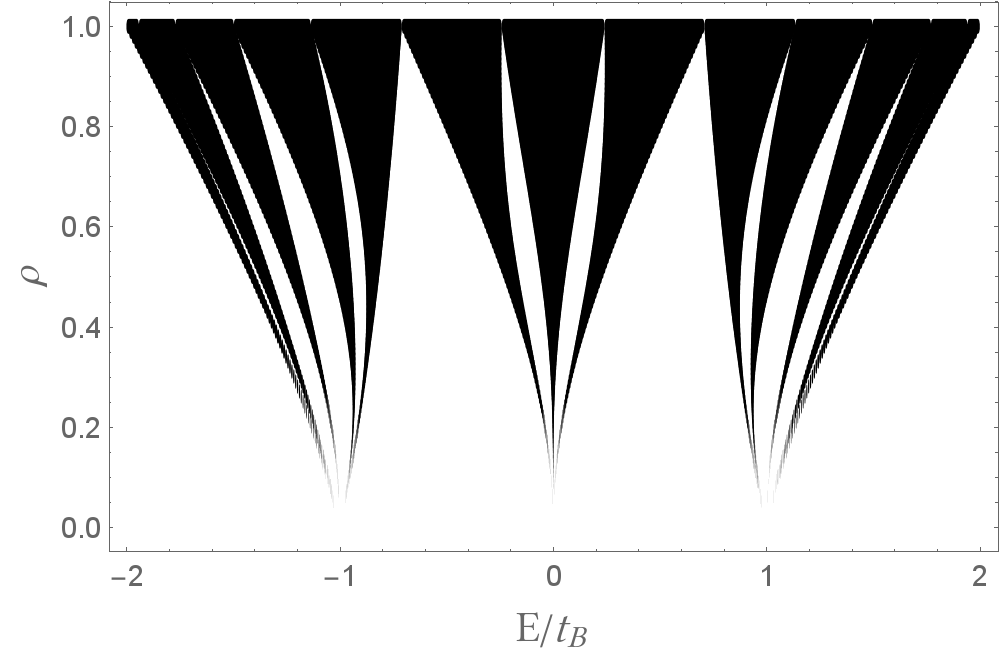
\includegraphics[width=.4\textwidth]{img/3_part2/fibonacci_spectra_varying_rho}

}

\end{frame}

\begin{frame}{Renormalization}
Substitution rule: $C_{l+1} = \sub(C_l)$ $\implies$ renormalization [Niu, Nori 86, Kalugin \etal{} 86]
	\begin{itemize}
	\item Atomic RG step (decimation of molecules) 
	
	{\centering
	\documentclass[talk.tex]{subfiles}
\begin{document}


    	\begin{tikzpicture}[scale=.7]
    		\newcommand{\orig}{-1.5}
    		\newcommand{\trans}{1.5}
    		\newcommand{\vertspac}{-2.}
    		\newcommand{\vertsize}{0} % vertical spand of the rectangles
    		\newcommand{\del}{.2}
    		\newcommand{\rad}{2pt} % radii of the circles
    	
    		% set the style of the strong bonds
    		\tikzset{
    			strong/.style={
    				double,
    				double distance=\rad,
    				line width=0.5pt
    				}
    		}
    		
    		% initial chain
    	
    		% bonds 
        	\draw[-] (\orig, 0)  node [left] {}  -- (\orig+\trans, 0)  node [midway, above] {$t_w$};
			\draw[strong] (\orig+\trans,0) -- (\orig+2*\trans,0)  node [midway, above] {$t_s$};
			\draw[-] (\orig+2*\trans,0) -- (\orig+3*\trans,0) node [midway, above] {$t_w$};	
			\draw[strong] (\orig+3*\trans,0) -- (\orig+4*\trans,0) node [midway, above] {$t_s$};
			\draw[-] (\orig+4*\trans,0) -- (\orig+5*\trans,0) node [midway, above] {$t_w$};
			\draw[-] (\orig+5*\trans,0) -- (\orig+6*\trans,0) node [midway, above] {$t_w$};
			\draw[strong] (\orig+6*\trans,0) -- (\orig+7*\trans,0) node [midway, above] {$t_s$};
			\draw[-] (\orig+7*\trans,0) -- (\orig+8*\trans,0) node [midway, above] {$t_w$};
    	
    		% sites
			\foreach \x in {0,...,7}
		      \filldraw (\orig+\x*\trans,0) circle (\rad); % node [below] {$\ket{\x}$};
		    % last site with chain step attached
		    \filldraw (\orig+8*\trans,0) circle (\rad) node [right] {~~~$n$};
		    
		    % rectangles around atoms
%		    \draw [rounded corners] (\orig-\vertsize,-\vertsize) rectangle (\orig+\vertsize,\vertsize);
%		    \draw [rounded corners] (\orig-\vertsize+5*\trans,-\vertsize) rectangle (\orig+\vertsize+5*\trans,\vertsize);
%		    \draw [rounded corners] (\orig-\vertsize+8*\trans,-\vertsize) rectangle (\orig+\vertsize+8*\trans,\vertsize);
		    
		    % arrows below rectangles
		    \draw [->] (\orig,-\vertsize-\del) -- (\orig,\vertspac+\del);
		    \draw [->] (\orig+5*\trans,-\vertsize-\del) -- (\orig+5*\trans,\vertspac+\del);
		    \draw [->] (\orig+8*\trans,-\vertsize-\del) -- (\orig+8*\trans,\vertspac+\del);
		      
		    % atomic chain
		    
        	\draw[-] (\orig, \vertspac)  node [left] {}  -- (\orig+5*\trans, \vertspac)  node [midway, above] {$\zb t_w$};
			\draw[strong] (\orig+5*\trans,\vertspac) -- (\orig+8*\trans,\vertspac) node [midway, above] {$\zb t_s$};
			
			\filldraw (\orig,\vertspac) circle (\rad); % node [below] {$\ket{\x}$};
			\filldraw (\orig+5*\trans,\vertspac) circle (\rad); % node [below] {$\ket{\x}$};
			\filldraw (\orig+8*\trans,\vertspac) circle (\rad) node [right] {~~~$n-3$};
		\end{tikzpicture}

\end{document}
	}
	
	\item Molecular RG step (decimation of atoms) 
	
	{\centering
	\documentclass[../fractal_dimensions_quasicrystals.tex]{subfiles}
\begin{document}


    	\begin{tikzpicture}[scale=.7]
    		\newcommand{\orig}{-1.5}
    		\newcommand{\trans}{1.5}
    		\newcommand{\vertspac}{-2.}
    		\newcommand{\vertsize}{0} % vertical span of the rectangles
    		\newcommand{\del}{.2}
    		\newcommand{\rad}{2pt} % radii of the circles

    		
    		% set the style of the strong bonds
    		\tikzset{
    			strong/.style={
    				double,
    				double distance=\rad,
    				line width=0.5pt
    				}
    		}
    	
    		% initial chain
    	
    		% bonds 
        	\draw[-] (\orig, 0)  node [left] {}  -- (\orig+\trans, 0) node [midway, above] {$t_w$};
			\draw[strong] (\orig+\trans,0) -- (\orig+2*\trans,0) node [midway, above] {$t_s$};
			\draw[-] (\orig+2*\trans,0) -- (\orig+3*\trans,0) node [midway, above] {$t_w$};	
			\draw[strong] (\orig+3*\trans,0) -- (\orig+4*\trans,0) node [midway, above] {$t_s$};
			\draw[-] (\orig+4*\trans,0) -- (\orig+5*\trans,0) node [midway, above] {$t_w$};
			\draw[-] (\orig+5*\trans,0) -- (\orig+6*\trans,0) node [midway, above] {$t_w$};
			\draw[strong] (\orig+6*\trans,0) -- (\orig+7*\trans,0) node [midway, above] {$t_s$};
			\draw[-] (\orig+7*\trans,0) -- (\orig+8*\trans,0) node [midway, above] {$t_w$};
    	
    		% sites
			\foreach \x in {0,...,8}
		      \filldraw (\orig+\x*\trans,0) circle (\rad); % node [below] {$\ket{\x}$};
		      
		    % rectangles around molecules
%		    \draw [rounded corners] (\orig +\trans-\del,-\vertsize) rectangle (\orig+2*\trans+\del,\vertsize);
%		    \draw [rounded corners] (\orig +3*\trans-\del,-\vertsize) rectangle (\orig+4*\trans+\del,\vertsize);
%		    \draw [rounded corners] (\orig +6*\trans-\del,-\vertsize) rectangle (\orig+7*\trans+\del,\vertsize);
		    
		    % arrows below rectangles
		    \draw [->] (\orig+1.5*\trans,-\vertsize-\del) -- (\orig+1.5*\trans,\vertspac+\del);
		    \draw [->] (\orig+3.5*\trans,-\vertsize-\del) -- (\orig+3.5*\trans,\vertspac+\del);
		    \draw [->] (\orig+6.5*\trans,-\vertsize-\del) -- (\orig+6.5*\trans,\vertspac+\del);
		      
			% molecular chains
			
			\foreach \x in {1}
			{
				\draw[-] (\orig, \x*\vertspac) node [left] {} -- (\orig+1.5*\trans, \x*\vertspac) node [midway, above] {$t_w'$};
				\draw[strong] (\orig+1.5*\trans, \x*\vertspac) -- (\orig+3.5*\trans, \x*\vertspac) node [midway, above] {$t_s'$};
				\draw[-] (\orig+3.5*\trans, \x*\vertspac) -- (\orig+6.5*\trans, \x*\vertspac) node [midway, above] {$t_w'$};
				\draw[strong] (\orig+6.5*\trans, \x*\vertspac) -- (\orig+8*\trans, \x*\vertspac) node [midway, above] {$t_s'$};
				
				\filldraw (\orig,\x*\vertspac) circle (\rad);
				\filldraw (\orig+1.5*\trans,\x*\vertspac) circle (\rad);
				\filldraw (\orig+3.5*\trans,\x*\vertspac) circle (\rad);
				\filldraw (\orig+6.5*\trans,\x*\vertspac) circle (\rad);
				\filldraw (\orig+8*\trans,\x*\vertspac) circle (\rad);
			}
		\end{tikzpicture}

\end{document}
	}
	
	\end{itemize}

	\flushleft{In the limit $\rho \ll 1$, $z= \rho/2$, $\zb = \rho^2$}
\end{frame}

\begin{frame}{RG construction \& renormalization paths}
 \[ H_l = \underbrace{\left( z H_{l-2} - t_s \right)}_{\text{\textcolor{BostonBlue}{bonding }levels}} + \underbrace{\left( \zb H_{l-3} \right)}_{\text{\textcolor{comp}{atomic} levels}} + \underbrace{\left( z H_{l-2} + t_s \right)}_{\text{\textcolor{BostonBlue}{antibonding} levels}} + \mathcal{O}(\rho^4)\]
	$\rightarrow$ recursive construction of the spectrum [Piéchon \etal{} 95]
	
	\begin{columns}
	\begin{column}{6cm}
	\centering
	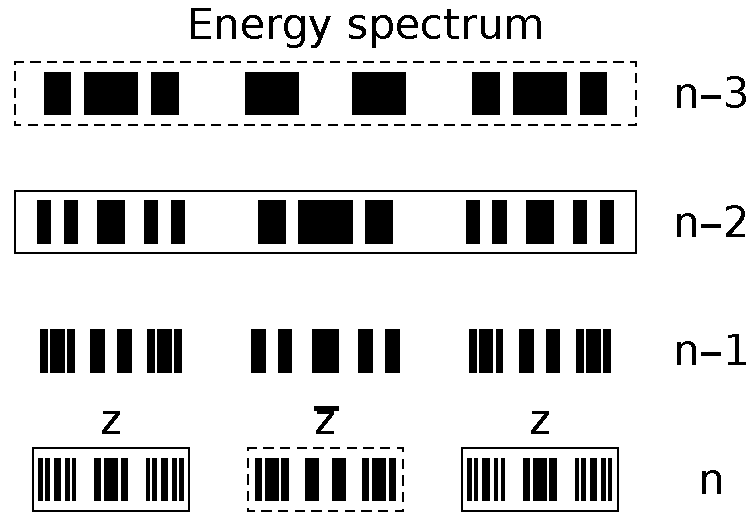
\includegraphics[scale=.4]{img/3_part2/recursive_construction_spectrum.pdf}
	\end{column}
	\begin{column}{6cm}
	Eigenstate $\leftrightarrow$ renormalization path:
	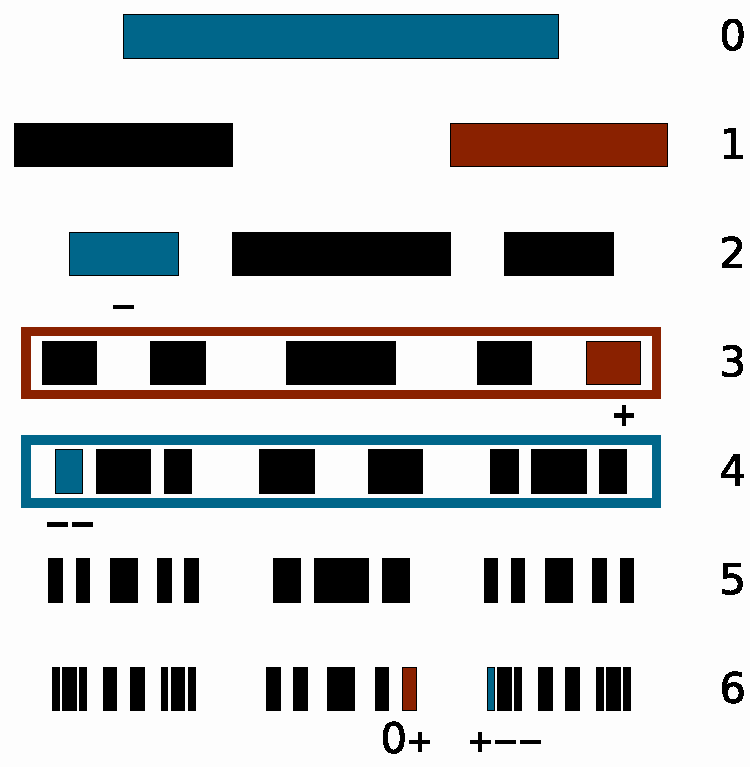
\includegraphics[scale=.3]{img/3_part2/renormalization_paths_spectrum.pdf}
	\end{column}
	\end{columns}
\end{frame}

%\begin{frame}{Perturbative RG for the wavefunctions}
%Substitution rule: $C_{l+1} = \sub(C_l)$ $\implies$ real space renormalization [Niu, Nori 86, Kalugin \etal{} 86, Macé \etal{} 16]
%	\begin{itemize}
%
%		\item Atomic RG (decimation of the molecules)
%			\begin{columns}
%			\begin{column}{9cm}
%				%\documentclass[talk.tex]{subfiles}
%\begin{document}


    	\begin{tikzpicture}[scale=.6]
    		\newcommand{\orig}{-1.5}
    		\newcommand{\trans}{1.5}
    		\newcommand{\vertspac}{-2.}
    		\newcommand{\del}{.2}
    		\newcommand{\rad}{2pt} % radii of the circles
    	
    		% set the style of the strong bonds
    		\tikzset{
    			strong/.style={
    				double,
    				double distance=\rad,
    				line width=0.5pt
    				}
    		}
    		
    		% initial chain
    	
    		% bonds 
        	\draw[-] (\orig, 0)  node [left] {}  -- (\orig+\trans, 0);%  node [midway, above] {$t_w$};
			\draw[strong] (\orig+\trans,0) -- (\orig+2*\trans,0);%  node [midway, above] {$t_s$};
			\draw[-] (\orig+2*\trans,0) -- (\orig+3*\trans,0);% node [midway, above] {$t_w$};	
			\draw[strong] (\orig+3*\trans,0) -- (\orig+4*\trans,0);% node [midway, above] {$t_s$};
			\draw[-] (\orig+4*\trans,0) -- (\orig+5*\trans,0);% node [midway, above] {$t_w$};
			\draw[-] (\orig+5*\trans,0) -- (\orig+6*\trans,0);% node [midway, above] {$t_w$};
			\draw[strong] (\orig+6*\trans,0) -- (\orig+7*\trans,0);% node [midway, above] {$t_s$};
			\draw[-] (\orig+7*\trans,0) -- (\orig+8*\trans,0);% node [midway, above] {$t_w$};
    	
    		% sites
			\foreach \x in {0,...,7}
		      \filldraw (\orig+\x*\trans,0) circle (\rad); % node [below] {$\ket{\x}$};
		     \filldraw (\orig+8*\trans,0) circle(\rad) node [right] {~~~$C_l$};
		      
		    \filldraw (\orig+5*\trans,0) circle (0) node [shift={(-0.4,0.3)}] {$|\psi_m|$};
		    
		    % vertical arrows
		    \draw [->] (\orig,-\del) -- (\orig,\vertspac+\del) node [midway, right] {$\lb$};
		    \draw [->] (\orig+5*\trans,-\del) -- (\orig+5*\trans,\vertspac+\del) node [midway, right] {$\lb$};
		    \draw [->] (\orig+8*\trans,-\del) -- (\orig+8*\trans,\vertspac+\del) node [midway, right] {$\lb$};
		    
		    % horizontal arrows
%			\path [->] (\orig+5*\trans,+\del)  edge [bend left=-90] (\orig+3.5*\trans,+\del);
%			\path [->] (\orig+5*\trans,+\del)  edge [bend left=90] (\orig+6.5*\trans,+\del);
%			\path [->] (\orig+5*\trans,+\del)  edge [bend left=-90] (\orig+1.5*\trans,+\del);
		      
		    % atomic chain
		    
        	\draw[-] (\orig, \vertspac)  node [left] {}  -- (\orig+5*\trans, \vertspac);%  node [midway, above] {$t_w'$};
			\draw[strong] (\orig+5*\trans,\vertspac) -- (\orig+8*\trans,\vertspac);% node [midway, above] {$t_s'$};
			
			\filldraw (\orig,\vertspac) circle (\rad); % node [below] {$\ket{\x}$};
			\filldraw (\orig+5*\trans,\vertspac) circle (\rad) node [shift={(-0.7,0.3)}] {$\sqrt{\lb} |\psi_{m}|$};
			\filldraw (\orig+8*\trans,\vertspac) circle (\rad)node [right] {~~~$C_{l-3}$};
		\end{tikzpicture}

%\end{document}
%			\end{column}
%			\begin{column}{2cm}
%			\[ \lb \simop{\rho \ll 1} \frac{1}{1+2\rho^2}
%			\]
%			\end{column}
%			\end{columns}
%		\item Molecular RG (decimation of the atoms)
%			\begin{columns}
%			\begin{column}{9cm}
%				\documentclass[talk.tex]{subfiles}
\begin{document}


    	\begin{tikzpicture}[scale=.6]
    		\newcommand{\orig}{-1.5}
    		\newcommand{\trans}{1.5}
    		\newcommand{\vertspac}{-2.}
    		\newcommand{\vertsize}{0} % vertical span of the rectangles
    		\newcommand{\del}{.2}
    		\newcommand{\rad}{2pt} % radii of the circles

    		
    		% set the style of the strong bonds
    		\tikzset{
    			strong/.style={
    				double,
    				double distance=\rad,
    				line width=0.5pt
    				}
    		}
    	
    		% initial chain
    	
    		% bonds 
        	\draw[-] (\orig, 0)  node [left] {}  -- (\orig+\trans, 0);
			\draw[strong] (\orig+\trans,0) -- (\orig+2*\trans,0);
			\draw[-] (\orig+2*\trans,0) -- (\orig+3*\trans,0);	
			\draw[strong] (\orig+3*\trans,0) -- (\orig+4*\trans,0);
			\draw[-] (\orig+4*\trans,0) -- (\orig+5*\trans,0);
			\draw[-] (\orig+5*\trans,0) -- (\orig+6*\trans,0);
			\draw[strong] (\orig+6*\trans,0) -- (\orig+7*\trans,0);
			\draw[-] (\orig+7*\trans,0) -- (\orig+8*\trans,0);
    	
    		% sites
			\foreach \x in {0,...,7}
		      \filldraw (\orig+\x*\trans,0) circle (\rad); % node [below] {$\ket{\x}$};
		     \filldraw (\orig+8*\trans,0) circle(\rad) node [right] {~~~$n$};
		     
		     \filldraw (\orig+3*\trans,0) circle (0) node [above] {$|\psi_i|$};
		    
		    % arrows below rectangles
		    \draw [->] (\orig+1.5*\trans,-\vertsize-\del) -- (\orig+1.5*\trans,\vertspac+\del) node [midway, right] {$\lambda$};
		    \draw [->] (\orig+3.5*\trans,-\vertsize-\del) -- (\orig+3.5*\trans,\vertspac+\del) node [midway, right] {$\lambda$};
		    \draw [->] (\orig+6.5*\trans,-\vertsize-\del) -- (\orig+6.5*\trans,\vertspac+\del) node [midway, right] {$\lambda$};
		      
			% molecular chains
			
				\draw[-] (\orig, \vertspac) node [left] {} -- (\orig+1.5*\trans, \vertspac);
				\draw[strong] (\orig+1.5*\trans,\vertspac) -- (\orig+3.5*\trans, \vertspac);
				\draw[-] (\orig+3.5*\trans, \vertspac) -- (\orig+6.5*\trans, \vertspac);
				\draw[strong] (\orig+6.5*\trans, \vertspac) -- (\orig+8*\trans, \vertspac);
				
				\filldraw (\orig,\vertspac) circle (\rad);
				\filldraw (\orig+1.5*\trans,\vertspac) circle (\rad);
				\filldraw (\orig+3.5*\trans,\vertspac) circle (\rad) node [shift={(-0.8,0.3)}] {$\sqrt{\lambda} |\psi_{i}|$};
				\filldraw (\orig+6.5*\trans,\vertspac) circle (\rad);
				\filldraw (\orig+8*\trans,\vertspac) circle (\rad) node [right] {~~~$n-2$};
			
		\end{tikzpicture}

\end{document}
%			\end{column}
%			\begin{column}{2cm}
%			\[ \lambda \simop{\rho \ll 1} \frac{1}{2+\rho^2}
%			\]
%			\end{column}
%			\end{columns}
%	\end{itemize}
%%\begin{align*}
%%		|\psi_m^{(l)}(E)|^2 &= \lb |\psi_{m'}^{(l-3)}(E')|^2 \text{~if $E$ is in the central cluster}\\
%%		|\psi_m^{(l)}(E)|^2 &= \lambda |\psi_{m'}^{(l-2)}(E')|^2 \text{~if }E\text{~is in the edge clusters}
%%\end{align*}
%\end{frame}

\begin{frame}{Fractality of the eigenstates}
RG $\to$ renormalization of the eigenstates [Macé \etal{} 16]
\begin{align*}
		|\psi_m^{(l)}(E)|^2 &= \textcolor{comp}{\lb} |\psi_{m'}^{(l-3)}(E')|^2 \text{~if $E$ \textcolor{comp}{atomic} level}\\
		|\psi_m^{(l)}(E)|^2 &= \textcolor{BostonBlue}{\lambda} |\psi_{m'}^{(l-2)}(E')|^2 \text{~if }E\text{~\textcolor{BostonBlue}{molecular} level}
\end{align*}

%Eigenstate $\leftrightarrow$ RG path


\(
\<{7cm}
Fractal dimensions of the eigenstates:
\[
d_q(x) = \frac{\log \Big[ \left( \frac{\lambda(\rho)^q}{\lambda(\rho^q)} \right)^x \left( \frac{\bar{\lambda}(\rho)^q}{\bar{\lambda}(\rho^q)} \right)^{(1-2x)/2} \Big]}{(q-1)\log \tau^{-1}}
\]

$x$: fraction of molecular RG steps in a path

$d_q(0)$: dimensions of the ``broccoli state''
\>
\<{7cm}
\centering
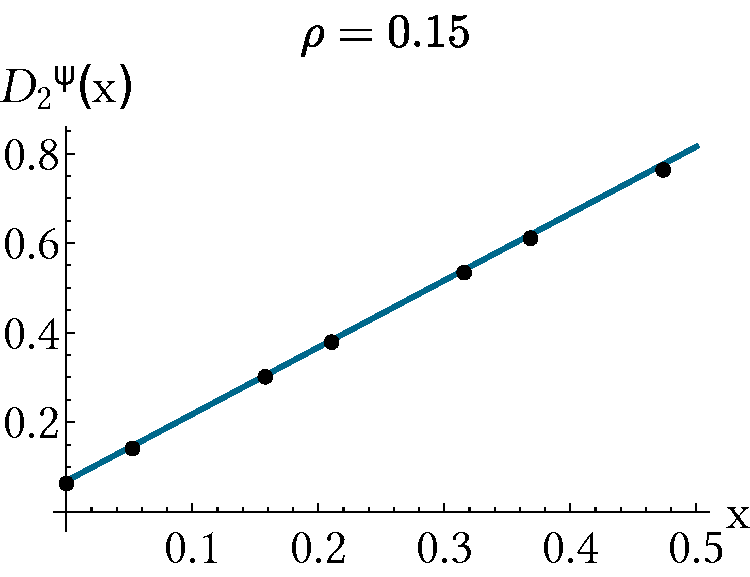
\includegraphics[width=.6\textwidth]{img/3_part2/local_wf}

{\ss Fractal dimensions for $\rho=0.15$: numerics \emph{vs} RG predictions}
\>
\)

\end{frame}

\begin{frame}{Conclusions}
Focus on the Fibonacci tight-binding chain, in the limit $\rho \ll 1$.
\begin{itemize}
	\item Substitution rule $\to$ scale invariance $\to$ renormalization group
	\item RG $\to$ eigenstates all \emph{fractal}
	\item Fractal dimensions depend only on $x$
\end{itemize}
\end{frame}
\section{2D eigenstates}
\subsection{Dummy}

\begin{frame}{Groundstate of the \AB\ tiling}
\(
\<{8cm}
\centering

\includegraphics[width=.8\textwidth]{img/4_part3/ammann}

{\ss A patch of the \AB\ tiling}
\>
\<{7cm}
Hamiltonian:
\[
	\op{H} = -t\sum_{\langle m,n\rangle} \ket{m}\bra{n}
\]
Quasiperiodicity encoded in adjacency and on-site potentials
\>
\)

\textbf{Fractal} states described by \textbf{height} functions?
\[
	\psi(m) = C(m) e^{\kappa h(m)}
\]
\end{frame}

\begin{frame}{Looking for arrows}
\(
\<{7cm}
Like Fibonacci, \AB\ has a substitution rule:

{\centering

\includegraphics[width=.8\textwidth]{img/4_part3/AB_inflation}
}

$\to$ scale invariance.

Height requires a field of arrows:
\begin{itemize}
	\item irrotational
	\item invariant under substitution
\end{itemize}
\>
\<{7cm}
\AB\ $\to$ notched tiles\dots

{\centering

\includegraphics[width=.7\textwidth]{img/4_part3/tiles_notches}

}

\dots exactly what we need!

{\centering
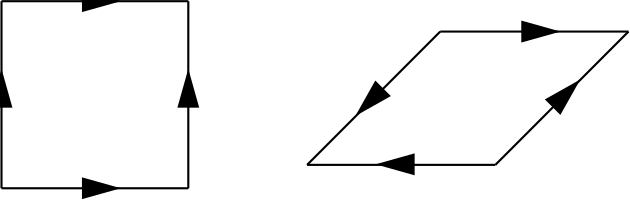
\includegraphics[width=.7\textwidth]{img/4_part3/tiles_arrows}

}

Height field:
\[
	h(m) = \sum_{0 \to m} \text{arrows}
\]
\>
\)
\end{frame}

\begin{frame}{Properties of the height field}

\(
\<{6cm}

{\centering
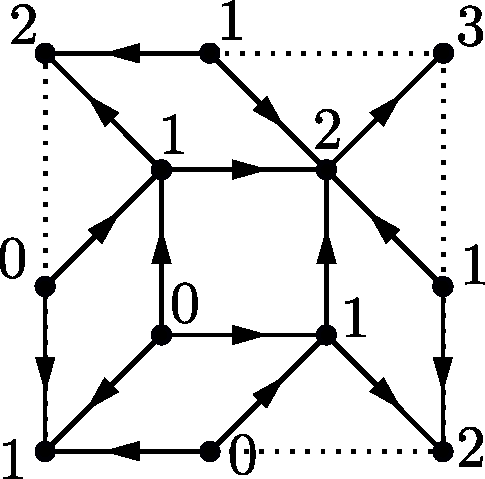
\includegraphics[width=.6\textwidth]{img/4_part3/heights_small_patch}

{\ss The height field on a small patch of the tiling.}

}

\>
\<{8cm}
{\centering
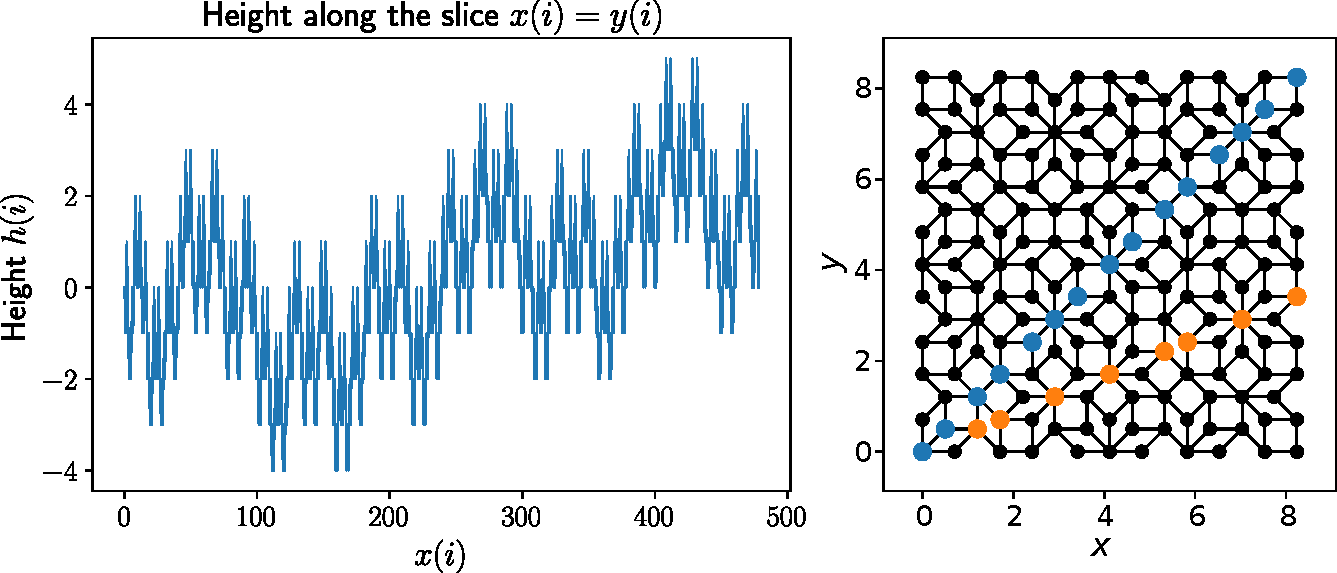
\includegraphics[width=1.\textwidth]{img/4_part3/height_combined}

{\ss Height along a line, shown in blue on the tiling.}

}

Partition function: $Z_L(\beta) \simop{L\to\infty} L^{\omega(\beta)}$

$\to$ slow growth: $h_\text{typ}(L) \simop{L\to \infty} \sqrt{\log L}$

$\to$ states $\psi(m) = e^{\kappa h(m)}$ fractal

\>
\)
\end{frame}

\begin{frame}{Groundstate}
\[
	\op{H} = -t\sum_{\langle m,n\rangle} \ket{m}\bra{n}
\]
Conjecture [Kalugin, Katz 14]:
\[
	\psi_\text{groundstate}(m) = C(m) e^{\kappa h(m)}
\]
\(
\<{7cm}
$C(m)$: \emph{local} function:

{\centering
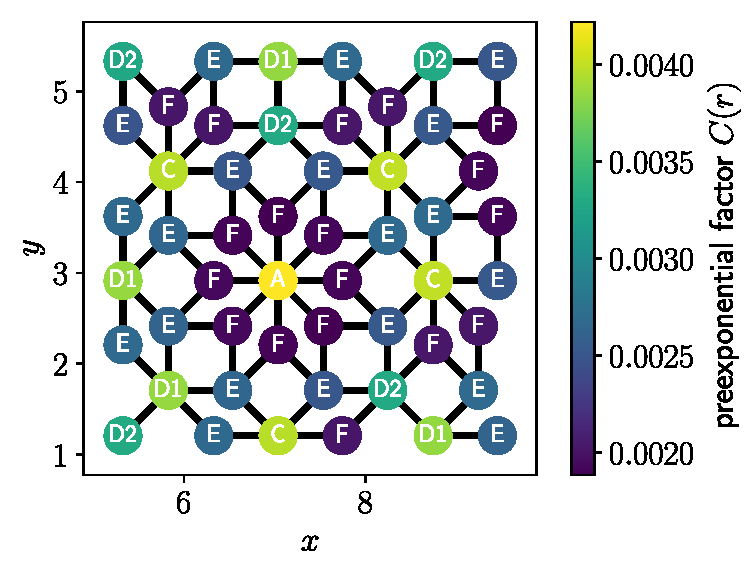
\includegraphics[width=.65\textwidth]{img/4_part3/SKK_cake}

}
\>
\<{7cm}
$e^{\kappa h(m)}$: non-local function:

{\centering
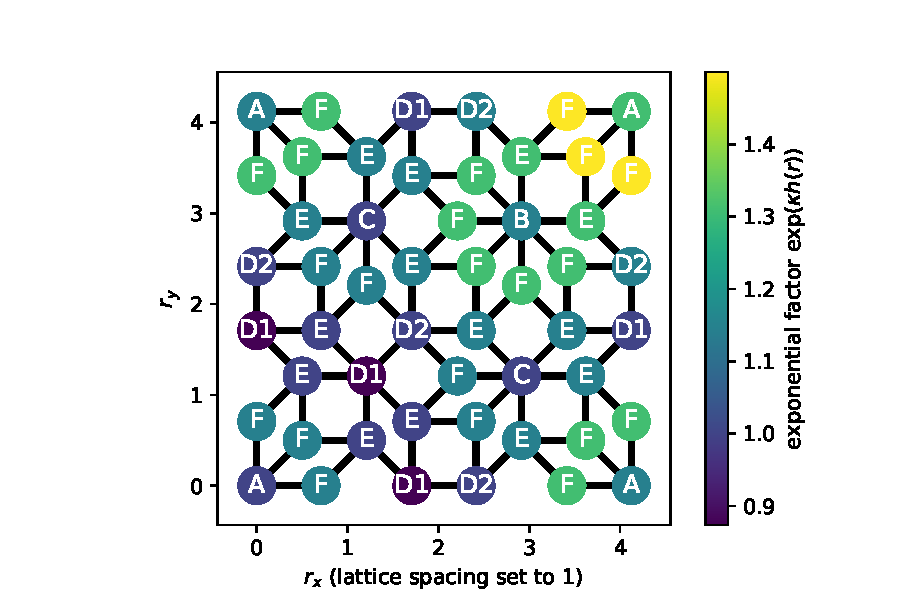
\includegraphics[width=.75\textwidth]{img/4_part3/SKK_exponential_2_para}

}

\>
\)
\end{frame}

\begin{frame}{Testing the conjecture}
Cut-and-project:

{\centering
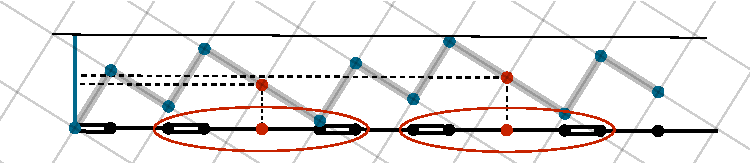
\includegraphics[width=.6\textwidth]{img/4_part3/cut_and_project_perp_projections}

{\ss Sites close in internal space have a very similar local environment.}

}
$\to$ internal space useful to test the local nature of $C$

\(
\<{5cm}
\centering
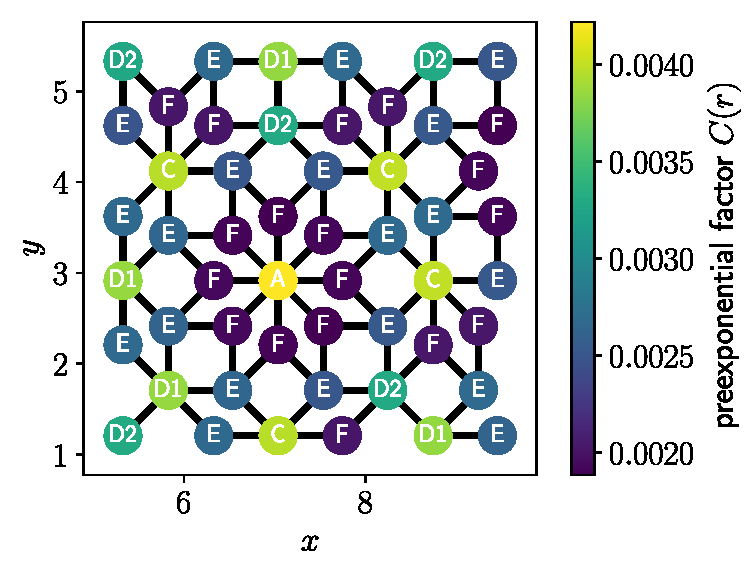
\includegraphics[width=1.\textwidth]{img/4_part3/SKK_cake}
\>
\<{5cm}
\centering
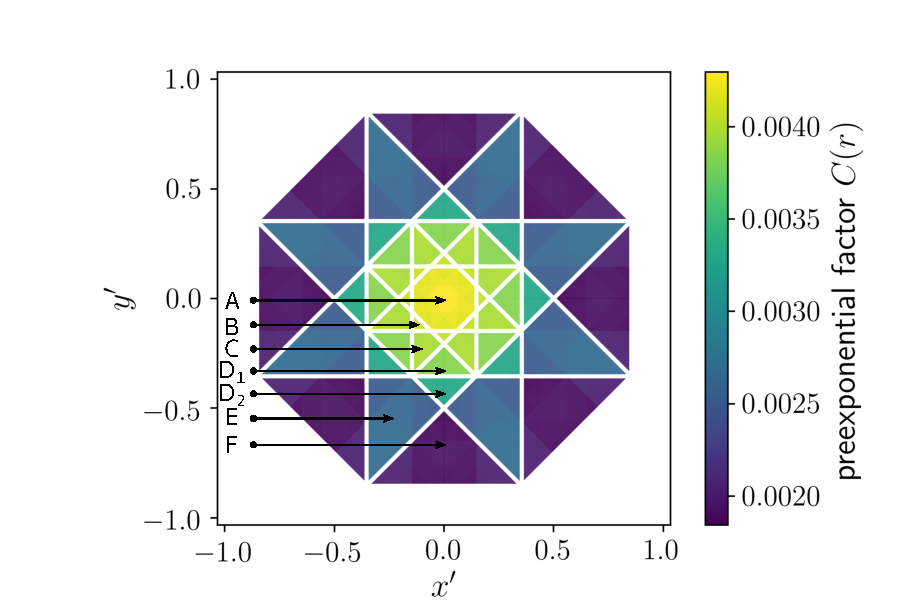
\includegraphics[width=1.\textwidth]{img/4_part3/14_SKK_cake_7_perp}
\>
\<{5cm}
\centering
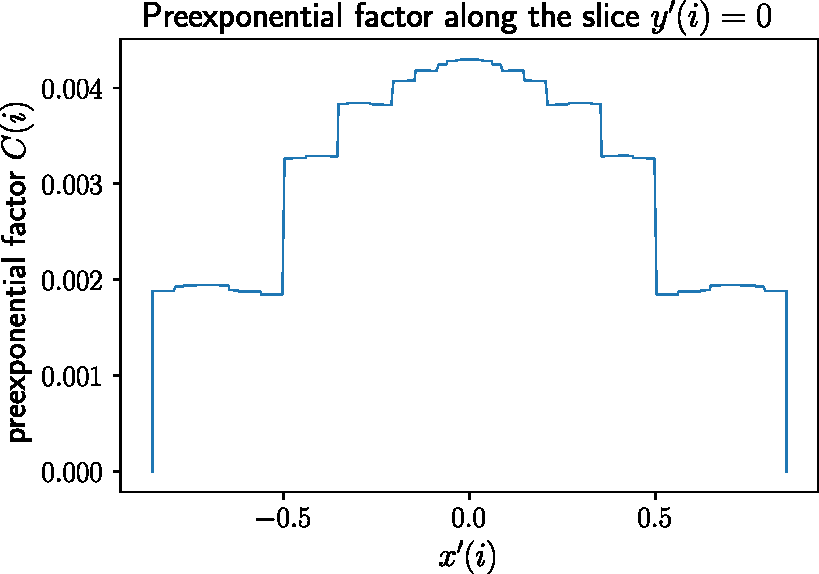
\includegraphics[width=1.\textwidth]{img/4_part3/15_SKK_cake_slice_7_perp}
\>
\)
\end{frame}

\begin{frame}{Perturbing the Hamiltonian}
Adding an on-site potential:
\[
	\op{H} = -t\sum_{\langle m,n\rangle} \ket{m}\bra{n} + \sum_m V_m \ket{m}\bra{m}
\]
\(
\<{7cm}
Laplacian-like [Sire, Bellissard 90]:
$V_m = V z_m$

$\to$ $\psi(m) = C(m) e^{\kappa h(m)}$

{\centering
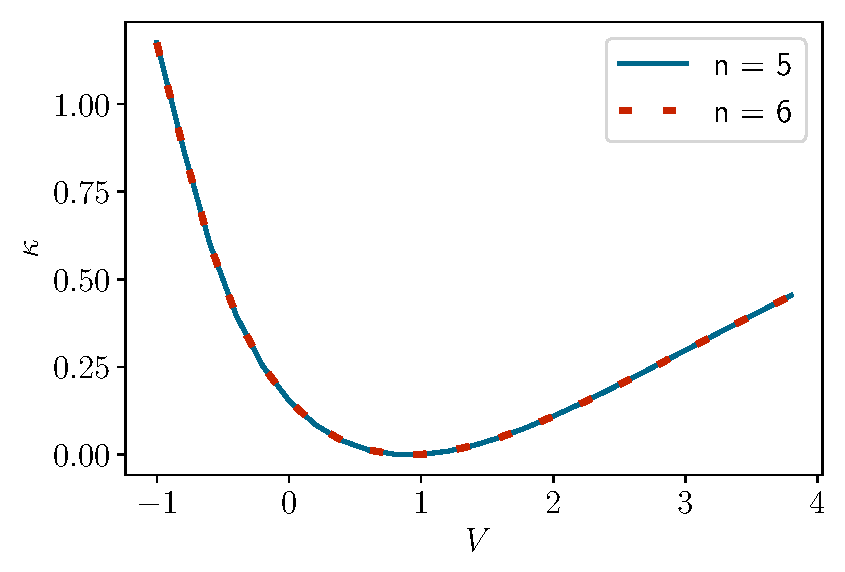
\includegraphics[width=.6\textwidth]{img/4_part3/kappa_n_5_6}

{\ss Prefactor $\kappa$ as a function of $V$.}

}

\>
\<{7cm}
An ``arbitrary'' potential:

$V_m = V$ if $m$ has 3 neighbors, else $V_m = 0$.

$\to$ $\psi(m) = C(m) e^{\kappa h(m)}$

{\centering
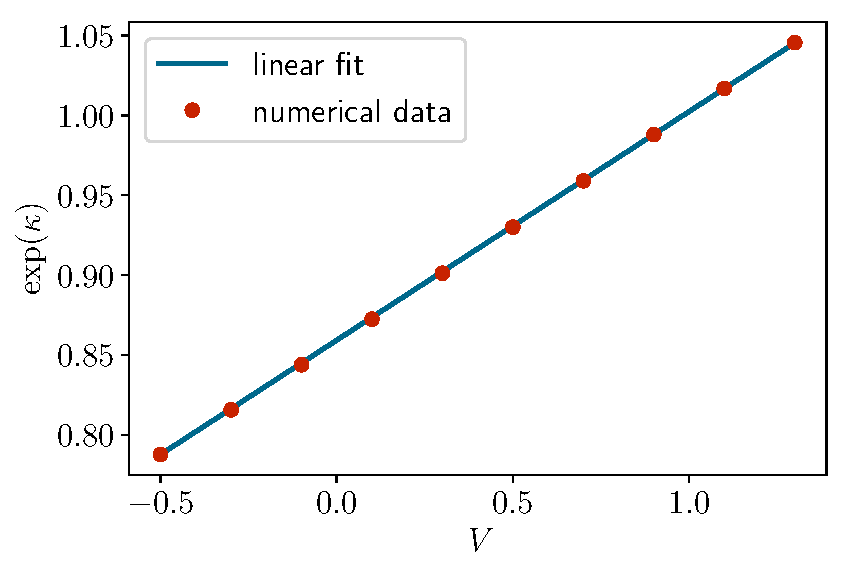
\includegraphics[width=.6\textwidth]{img/4_part3/beta_customF_ham}

{\ss{$e^{\kappa}$ as a function of $V$.}}

}

\>
\)
\end{frame}

\begin{frame}{Conclusions}
Tight-binding models on a 2D quasiperiodic tiling
\begin{itemize}
	\item Geometry (notches) $\to$ \textbf{height field} $h(m)$ $\to$ $\psi_\text{groundstate}(m) = C(m) e^{\kappa h(m)}$
	\item Slow height growth ($h(L) \sim \sqrt{\log L})$ $\to$ critical, \textbf{fractal} state
	\item Robust to symmetry-preserving on-site perturbations
	\item Same conclusions for the 10-fold symmetric Penrose tiling.
\end{itemize}
\end{frame}

\begin{frame}{General conclusion}
Simple tight-binding models on 1D and 2D quasiperiodic tilings
\begin{itemize}
	\item Quasiperiodic structures: in between periodic and random
	\item Critical, fractal eigenstates
	\item Consequence of quasiperiodic geometry
\end{itemize}
Perspectives
\begin{itemize}
	\item
\end{itemize}
\end{frame}

\end{document}